\documentclass[a4paper,english]{book}
\usepackage[utf8]{inputenc}         % or whatever you use

\usepackage[T1]{fontenc, url} %andreas
%\usepackage[T1]{url}
\urlstyle{sf}
\usepackage{ifipackages/ifikompendiumforside}
\usepackage{textcomp} %andreas slutt

\usepackage{graphicx, wrapfig}
%\usepackage{caption}
\usepackage{booktabs}
\usepackage[labelfont=it,textfont=it]{caption}
\usepackage{subcaption}
\usepackage{amsmath,amsfonts,amssymb}
\usepackage[hypcap]{caption}
\usepackage{xcolor,colortbl}
\usepackage{mathtools}
\usepackage{multirow}
\usepackage{array}
\usepackage{fancyvrb, babel, csquotes, varioref, graphicx}
%\usepackage{fancyvrb, csquotes, varioref, graphicx}
\usepackage{float}
%\floatstyle{plaintop}
\restylefloat{table}
\usepackage[section]{placeins}
\usepackage{tabularx}
\usepackage{listings}
%\usepackage{subcaption}
\usepackage{comment}
%\usepackage[caption=false]{subfig}
\usepackage{hyperref, enumitem}

%\usepackage[romanian]{babel}
\usepackage{combelow}
\usepackage{layout}
\usepackage{hhline}
\usepackage{dcolumn}
%\usepackage[sorting=none, backend=bibtex]{biblatex}
\usepackage[style=numeric,backend=bibtex]{biblatex}
%\usepackage{flushright}
%\usepackage{multibib}
%\newcites{wikipedia}{Wikipedia References}%


\addbibresource{mybib.bib}

\makeatletter
%\renewcommand{\@chapapp}{}% Not necessary...
\newenvironment{chapquote}[2][2.5em]
  {\setlength{\@tempdima}{#1}%
   \def\chapquote@author{#2}%
   \parshape 1 \@tempdima \dimexpr\textwidth-2\@tempdima\relax%
   \itshape}
  {\par\normalfont\hfill--\ \chapquote@author\hspace*{\@tempdima}\par\bigskip}
\makeatother


%\usepackage{amsmath,amssymb}
\makeatletter
\newsavebox\myboxA
\newsavebox\myboxB
\newlength\mylenA

\newcommand*\xoverline[2][0.75]{%
    \sbox{\myboxA}{$\m@th#2$}%
    \setbox\myboxB\null% Phantom box
    \ht\myboxB=\ht\myboxA%
    \dp\myboxB=\dp\myboxA%
    \wd\myboxB=#1\wd\myboxA% Scale phantom
    \sbox\myboxB{$\m@th\overline{\copy\myboxB}$}%  Overlined phantom
    \setlength\mylenA{\the\wd\myboxA}%   calc width diff
    \addtolength\mylenA{-\the\wd\myboxB}%
    \ifdim\wd\myboxB<\wd\myboxA%
       \rlap{\hskip 0.5\mylenA\usebox\myboxB}{\usebox\myboxA}%
    \else
        \hskip -0.5\mylenA\rlap{\usebox\myboxA}{\hskip 0.5\mylenA\usebox\myboxB}%
    \fi}
\makeatother

%\usepackage[margin=0.5in]{geometry}
\hypersetup{
    linktocpage,
    colorlinks, 
    citecolor=black, 
    filecolor=black,
    linkcolor=black,
    urlcolor=black,
    linktoc=all
    }

%\floatsetup[table]{capposition=top}
\DefineVerbatimEnvironment{code}{Verbatim}{fontsize=\small}

% The programs I have made
\newcommand{\catlinkprogram}{\texttt{Split\_catlink.py} }
\newcommand{\catgraphbuilderprogram}{\texttt{Categorygraph\_builder.py} }
\newcommand{\artbuildprogram}{\texttt{}}

\newcommand\Chapter[2]{
  \chapter[#1: {\itshape#2}]{#1\\[2ex]\Large\itshape#2}
}

\renewcommand{\lstlistingname}{Code}
\lstdefinestyle{customasm}{
  basicstyle=\ttfamily,
  belowcaptionskip=1\baselineskip,
  frame=trLb}

\lstset{ captionpos=b, style=customasm, xleftmargin=\parindent,breaklines=true,}
% aboveskip=20pt,belowskip=20pt,  
% own environment for code
%\newcounter{codecnt}
%\labelformat{codecnt}{Code~#1}


\newcommand*\justify{%
  \fontdimen2\font=0.4em% interword space
  \fontdimen3\font=0.2em% interword stretch
  \fontdimen4\font=0.1em% interword shrink
  \fontdimen7\font=0.1em% extra space
  \hyphenchar\font=`\-% allowing hyphenation
}

\newcommand{\enwikipageprops}{\texttt{\justify{enwiki-latest-page\_props.sql.gz}}}
\newcommand{\enwikipage}{\texttt{\justify{enwiki-latest-page.sql.gz}}}
\newcommand{\enwikicatlink}{\texttt{\justify{enwiki-latest-categorylinks.sql.gz}}}
\newcommand{\allhidden}{\texttt{\justify{All\_hidden\_categories.txt.gz}}}
\newcommand{\enwikiredirect}{\texttt{\justify{enwiki-latest-redirect.sql.gz}}}
\newcommand{\outputredirect}{\texttt{\justify{output-redirect-titles.txt.gz}}}
\newcommand{\subcat}{\texttt{\justify{Sub-categories.txt.gz}}}
\newcommand{\pagecat}{\texttt{\justify{Page-categories.txt.gz}}}
\newcommand{\subcatlink}{\texttt{\justify{Subcat\_links.txt.gz}}}
\newcommand{\catinfo}{\texttt{\justify{category-info.txt}}}
\newcommand{\artinfo}{\texttt{\justify{article-info.txt.gz}}}
\newcommand{\enwikicategory}{\texttt{\justify{enwiki-latest-category.sql.gz}}}
\newcommand{\enwikilanglinks}{\texttt{\justify{enwiki-latest-langlinks.sql.gz}}}

\newcommand{\enwikidatabasedumps}{\texttt{\justify http://dumps.wikimedia.org/enwiki}}
\newcommand{\ingridthesis}{\texttt{\justify https://github.com/ingridguren/Master-Thesis-2015}}




\title{Content Categorization for Contextual Advertising Using Wikipedia}
\author{Ingrid Grønlie Guren}

%\bibliography{mybib}

\begin{document}
%\ififorside{}

\ififorside
\frontmatter{}
\maketitle{}


\chapter*{Abstract}
Automatic categorization of content is an important %piece of 
functionality in online advertising and automated content recommendations, both for ensuring contextual relevancy of placements and for building up behavioral profiles for users that consume the content. Within the advertising domain, the taxonomy tree that content is classified into is defined with some commercial application in mind and needs to somehow reflect the advertising platform’s ad inventory. The nature of the ad inventory and the language of the content might vary across brokers (i.e., the operator of the advertising platform), so it is of interest to develop a system that can easily bootstrap the development of a well-working classifier. Brokers are often not very technical and by experience will have severe problems developing training sets or otherwise contribute to the process, so any required involvement from their side has to be relatively simple. Furthermore, it is a practical requirement that the classifier can “explain” its classification to the broker in some way, and that the broker can have a simple way to manually override or influence the classification of known problem cases.

We explore the use of Wikipedia to develop a simple dictionary-based classifier. A dictionary-based classifier offers a simple way to “explain” the classification, and allows the classification vocabulary (i.e., the dictionary entries) to be easily edited. Wikipedia exists in a large number of languages, has a large number of article keywords covering most domains, and explicitly associates article names with categories. We describe a set of tools that automate the process of building up dictionaries that map Wikipedia keywords (or cleansed versions thereof) into Wikipedia categories (or modified versions thereof). Creating a mapping that maps Wikipedia categories into the broker’s custom taxonomy tree is a relatively straightforward task that brokers (or people working on their behalf) are assumed capable of. We will here use predefined a taxonomy, the one provided by IAB, as a working example of such a custom taxonomy tree.

Given such a classifier, we describe an experiment using a real advertising platform to validate its use in real life using real data. We also provide a brief overview of related work described in the literature.
\chapter*{Acknowledgements}
This study has been a project for Xcense (\url{http://www.cxense.com}) and the Department of Informatics at the University of Oslo, and was started in the Spring semester 2014 and finished ** 2015. 

I would like to express my gratitude to my supervisor Aleksander Øhrn for all his incredibly important feedback and for all the advices he has given me through the process. 
%all advices he has given me and his scrunity of my thesis. 
I would also like to thank Gisle Ytrestøl for all his help, including all the quick responses on email, long discussions about implementations and his never-ending support and optimism about the project. 

Finally I would like to thank my family and study friends for all help, comments and discussions, and most important for supporting me every day. I could never have done this without any of you.   
\pagenumbering{roman}
\tableofcontents{}
\listoffigures{}
\listoftables{}

\pagenumbering{arabic}
\mainmatter{}
%\pagenumbering{arabic}
[Input Introduction here].
\chapter{Background}

\section{Automatic Content Analysis}
\label{sec:automatic_content_analysis}

\subsection{What is Content Analysis?}
Content analysis is the task of analysing and understanding collections of texts, in other words finding out what a text "is about". The task can be performed by both humans (manual content analysis) and computers (automatic content analysis), and both of the approaches have their advantages and disadvantages.

The concept of manual content analysis is easy. The task is split into first reading and understanding the text, then summarizing the content of the text and/or categorizing it into suitable categories describing the content. As an example, an article about \emph{Ole-Johan Dahl} (the famous Norwegian computer scientist \cite{Olejohandahleng}) would probably be summarized as an article about a famous Norwegian computer scientist and might be categorized under the category \emph{Norwegian computer scientists} if this category is present or the category \emph{computer scientists} if this is present.  
%as an article about authors of children books and Swedish people. 
There are two main disadvantages of manual content analysis which makes it impossible to perform on large collections of texts. The first disadvantage is that the task is time consuming, i.e. it takes time for a human to read and understand an article. The second disadvantage is that manual content analysis requires resources that might be expensive, for instance experts needed for understanding the content of an article if the article is about something beyond common knowledge.

%because some articles needs experts for understanding the content. 
%first has to be read and understood and then we could summarize the content of the text or categorize it under relevant topics.
Automatic content analysis is based on a different approach; instead of reading and understanding the text, the machine looks for predefined properties of the text (in our case known words or phrases) and uses these properties to determine the meaning of the text. This requires some predefined connection between the properties and their associated categories. This approach has disadvantages as well; computers lack commonsense knowledge usually known to ordinary humans, for instance physical description or function of objects. % TODO: Insert reference here.
Color is an example of a physical description computers have problems with determine. Most humans would understand that the phrase \emph{same color as the sun} means yellow, while computers would need specific information about the sun being yellow to conclude the same. 

Another disadvantage with automatic content analysis is dealing with disambiguation. Some words have more than one meaning, and the meaning is usually found from the context or the other words in the sentence. The task of determining the true meaning of a word or sentence is a difficult process which becomes harder if the sentences are complex. 

% TODO: Insert example of complex sentence.

%The easiest way to describe the meaning of the text is to group texts with similar content together, in other word categorize the texts. 

%Some of the advantages with automatic content analysis are that miss


%There are different ways to perform automatic content analysis, our approach is to find the most likely category for texts given as input by first categorizing all articles from Wikipedia. 

%involves using categorization of articles from Wikipedia to determine 

\subsection{Domain of Content Analysis}
Automatic content analysis can be found useful in many different settings, but the 
%There are many areas where content analysis (the task of understanding the content of the text) is useful, but the 
two most dominating areas are advertising and improvement of user experience. The focus for this project is to improve advertising and is therefore the main domain.
%Content analysis is useful for understanding texts, and is often used in two domains; advertising and improving user experience. 

Advertising is the main income of most online companies that provide free services. Many online companies provide their services for free, but make their money on advertisement instead. The alternative to this is to charge users a fee, before they are allowed to use the services. The online market is very competitive and most users expect everything on the Internet to be free. The most common approach is therefore to provide the services for free, but earn money on advertising instead. 

%free services with advertisement is to sell access to to their services, 

%but this is in many cases not possible because the online market is very competitive and many users expect everything on the Internet to be free. 

%difficult in many cases because of how competitive the market is and the expectations of a free Internet. 
%Online advertising is a growing market and is the main income of many online companies. 
%Online companies have two ways of earning money, they could either let the user pay to use the services or earn money on advertisement. Most web pages choose the second option because the market is very competitive and many web users expects the web pages to be free. %A newspaper might loose readers when trying to charge them. 

%Hence the companies have to earn money without charging the user for their services, and in most cases  this leads to advertisement. 
There are different approaches of doing advertisement on web pages. The most common ones are PPC (pay per click) and CPM (cost per mille). CPM is an  advertising technique where the advertiser pays for showing the page to a crowd, while PPC means that an advertisement is shown and the advertiser has to pay for each time a user clicks on the advertisement. Both of the techniques are more valuable for all parts if the advertises are shown to people that are interested and more likely to buy their product. The advertiser has a greater chance of getting customers if the advertisement is shown to the right crowd and the publisher can charge a higher price for the advertisement if the advertiser is more pleased with the result of the advertises.

The main advantage of specified advertisement is that the advertisement can be directed towards users that are more likely to become customers. This means that the advertiser needs to know the users and their interests. Content analysis can be part of building up a profile of the user, since knowing the content of user's text can provide information of the interests of the users. 


\section{Categorization}
Categorization is the process of grouping collections of text into categories, and can be done by both humans or computers. Computer categorization is the technique of teaching a classifier how to decide the category of any input \cite{wiki:categorization}. The idea of this process is to find patterns which makes the machine able to predict the category or class of the input. Such patterns could be similarities between input or decision rules \cite{wiki:classification}. It is desirable to optimize the results of the classifier so that the classifier is as accurate as possible. This can be done by learning the classifier how to behave, either by machine learning where the classifier optimizes itself based on feedback, or by improving the classifier's decision rules.  \\\\
%make the classifier as good as possible,
%Categorization with machine learning can be split into further types; statistical classification which is a \emph{supervised} learning process, and clustering which can be performed as both %an \textit{supervised} and a \emph{supervised} and an \emph{unsupervised} learning process. Supervised learning is a technique where the machine is given a training data set, where the set contains the correct output in addition to the input we want to classify. The classifier uses this data to learn the machine how to behave, also called training the classifier. Unsupervised learning, on the other hand, is the task of trying to find a hidden structure in unlabeled data. The main difference between the two types is that unlabeled data gives no feedback to the classifier, hence the classifier has to assume that it is correctly classified without receiving feedback. It is also possible to have classification processes which are combined of the two, where prior knowledge is given to the classifier. 
%added to the classification process for better results. 
%the data is unlabeled is no feedback sent to the classifier. 
%The classifier will therefore not know if the result is correct, but will continue to classify assuming that the classification performed so far is correct.  
Our problem consists of two categorization problems: 
\begin{enumerate}
\item Categorization of keywords.
\item Categorization of any text.
\end{enumerate}

%the main categorization where any article given as input should be categorized to its most describing category.  

\subsubsection{Categorization of keywords}
The categorization of keywords is done by creating a keyword list based on titles of Wikipedia articles. These keywords have to be categorized to suitable output categories. This categorization could be split into two parts: 

\begin{enumerate}
\item Categorize the keywords to Wikipedia categories represented as category paths  (see figure \ref{fig:keywords_to_categories}). This categorization should be based on the content of the Wikipedia articles of the keywords. Our assumption is that the meaning of a Wikipedia article can be found by looking at the underlying structure of Wikipedia, i.e., the article's categories and the category structure.\begin{figure}[h]
\centering

\includegraphics[width=0.4\textwidth]{Chapters/Background/Keywords_to_categories}
\caption[Categorization of keywords to Wikipedia categories]{Illustration of the categorization of keywords to Wikipedia categories.}
\label{fig:keywords_to_categories}
\end{figure}
\item The complete categorization of the keywords are based on creating a connection between the keywords and categories from IAB's taxonomy (see figure \ref{fig:keywords_categorization_full}). This categorization is based on rules between excerpts of Wikipedia category paths and the output categories. 
\begin{figure}[h]
\centering

\includegraphics[width=0.7\textwidth]{Chapters/Background/Keywords_categorization_full}
\caption[Categorzation process of the keywords]{Illustration of the complete categorization process of the keywords.}
\label{fig:keywords_categorization_full}
\end{figure}
\end{enumerate}
%the categorization by finding rules and apply heuristics. 

%The categorization needed to determine the categories for each article is a statistical classification. Wikipedia's structure is available and this can be used to find the most likely categories. 

\subsubsection{Categorization of any text}
The goal for this project is to be able to categorize any text based on the results from the categorization of the keywords. The classifier for this categorization process needs some rules on how it should classify. Our theory is that occurrences of keywords can determine the content of the text, and multiple keywords categorized to the same category indicate that the text should be categorized to this category. Thus, the classifier needs a way of detecting keywords in the text and a way of determining which category the text belongs to if it contains keywords from different categories. 


%. The main assumption 

%The next classification problem is to classify 
%Our main assumption for content analysis is that articles which contains the same keywords also belong to some of the same categories in Wikipedia. This means that we want create a group of these articles so that similar articles are grouped together. Supervised classification requires, as already mentioned, a training set. The training set of our problem can be defined as articles in Wikipedia since they are already connected to a category within Wikipedia. The task is to create the classifier that use  this information and is able to classify all other articles. 

%does not have a training set because it is almost impossible to create a training set representiing such a large data set. We still have, however,  information about the underlying category structure of the articles in Wikipedia. The goal is therefore to use this information to group similar articles together.
%Our problem is not suitable for supervised machine learning. Trying to solve the problem with supervised classification would lead to some problems that are difficult to solve; it is for instance almost impossible to create a training set to represent such a large data set and it is therefore not possible to create a classification model based on the data. The categorization should therefore be done with unsupervised machine learning, for instance clustering.

%The formal definition of cluster analysis or clustering is the task of grouping similar elements together.Hence the group or cluster should contain elements that share similarities or that are more similar to each other than to the rest of the elements. %This means that elements within a group are more similar to each other than to the rest of the elements, or that the elements within the group have some similarities that make them stand out from the others. 
%Our problem could therefore be defined as a clustering problem, where each cluster or group is the articles which contains some of the same keywords. We want to sort the texts in such a way that texts with similar content are classified to the same cluster and therefore to same category. The problem needs a mapping process so that collections of texts get clustered together within the predefined set of categories. The predefined set of categories will change depending on the purpose of the classification, for instance would advertisement need a different set of categories than categorization of news articles. A proposal to a predefined category set for advertisement is the category set of IAB. 
\section{Wikipedia}
%It has already been mentioned that content analysis needs a keyword list for recognizing words or phrases that are useful for classification. We require that the list is so large that it contains almost all the words that give information of possible categories for the content where the keyword is found.  We have chosen to use Wikipedia to create such a keyword list. 
Wikipedia is a free, online encyclopedia and community that was created by Jimmy Wales in 2001. The encyclopedia is edited by the Wiki-principle, which means that everyone can create and edit articles. To understand the importance of Wikipedia it is worth mentioning that the web page has been ranked as the fifth globally most important web page (New York Times, February 2014), with more than  30 million articles and almost 500 unique users a month. 

Wikipedia contains lots of articles within many subjetcs and is maintained by thousands of people. 
%is a good choice for a base for the keyword list since it contains lots of articles within many subjects and is maintained by thousands of people. 
Hence the idea is to base the list on all the titles in Wikipedia, but the list has to be modified to contain only relevant titles. It is for instance not relevant to have common words in the keyword list which will occur in most articles and not provide any useful information. 
%, like "the" for example, because these will not provide any useful information. 
It is also important to remove or weight down ambiguous words, i.e. words that could confuse the categorization process or apply wrong information. 

One of the main advantages of using Wikipedia is the underlying structure that is already provided. All articles are already categorized which gives information about the content of the article connected to the title. 

%There are many advantages of using Wikipedia, one of them is that all articles are already categorized which gives information about a possible category for each category. This means that the process of mapping between keyword and category  easily can be done by the computer. Another advantage is that it contains articles within various fields and is well maintained.

\subsection{Structure of Wikipedia}
The structure of Wikipedia is web based, where articles with similarities are linked together. Since Wikipedia is language-based, articles only link to other articles within the same language. Wikipedia does also have a category structure, where all articles are classified under at least one category. A category could have articles, but could also have subcategories, where the subcategories have their own articles and subcategories. All the categories form a large category graph where articles are put under the most describing categories, as an example is Ole Johan Dahl \cite{Olejohandahleng} (Norwegian computer scientist) placed under the category \emph{Norwegian computer scientists} instead of the parent category \emph{Computer scientists by nationality} or \emph{Computer Scientists}. 

The category graph is created so there is a link between a category and its subcategories. There is no beginning of the category graph, but here are some categories which have most other categories as their subcategories. These can be though of as beginning categories, also called root categories, and are important when we want to look through all categories in the graph and observe the relationships between them.  Two categories that can be viewed as potential root categories are \emph{Fundamental Categories} or \emph{Main Topic Classifications}. If one of these are chosen as the root category, we can continue through the graph by looking at its subcategories and proceed by looking at each of the subcategory's subcategories an so on.
%An important 
%The easiest way of looking at all categories in the graph is to choose a root category and follow the links to its subcategories and then continue to look 

Figure \ref{fig: subcat_lindgren} is an example of a structure for the category \emph{Astrid Lindgren}, the swedish children's writer. The figure shows a tree structure for the category from the category graph. The figure shows that the category \emph{Astrid Lindgren} has 10 pages directly under the category, and 4 subcategories: \emph{Astrid Lindgrens characters} (9 pages), \emph{Films based on works by Astrid Lindgren} (1 subcategory and 23 pages), \emph{Works by Astrid Lindgren} (2 subcategories and 7 pages) and \emph{Pippi Longstocking} (1 subcategory and 10pages).  This means that there are indirectly 59 pages under the category \emph{Astrid Lindgren} whithout counting pages under the next level of subcategories. 


%is created and how it is fetched from the page for category information.\footnote{\categorytree}

\begin{figure}[H]
\centering

\includegraphics[height=2.5cm]{Chapters/Background/Astrid_Lindgren}
\caption{Subcategories of the category \emph{Astrid Lindgren}. }
\label{fig: subcat_lindgren}
\end{figure}

% HVORFOR IKKE BRUKE WIKIPEDIA SINE KATEGORIER!
Wikipedia articles are already classified under categories, but the set containing all Wikipedia categories cannot be used as a final categorization. The category set in Wikipedia is too large for such usage, where some categories do not provide information of the actual content, and some are too specified. There are also cases where articles are categorized under categories where the combination of the categories does not provide any new information. An example is the article of \emph{Ole Johan Dahl}. Some of the article's categories are showed in figure \ref{fig: olejohandahl_categories}. In this example is the article both placed in the catgory \emph{People from Mandal, Norway} and in the category \emph{Norwegian Computer Scientists}. These categories both provide information about him being Norwegian, so it would be sufficient to put him in the category \emph{Computer Scientists}. The categories are also shown are also quite specific, and it might be desirable with more general categories. 


%of an article where the categories provide the same information, i.e., we already know that he was from Norway since he is in the category \emph{People from Mandal, Norway}, so it would be enough to add that he was a computer scientist instead of specifying that he was a Norwegian computer scientist. 

%categorization between articles and categories cannot be used as a pre-defined category set. 
%Another reason for creating a new independent category set is that Wikipedia categories are not guaranteed to be in the desirable final category set. 

Another reason for creating a new independent category set is that the Wikipedia categories are not guaranteed to be in the desirable final category set. Hence it is essential that the classifier creates a connection from the article and to a category that is know to exist in the set. The classifier should instead be based on the category information provided by Wikipedia. 

%We will therefore need a mapper to a category we know exists. 
%but we cannot use either the categorization from articles to categories nor 
%this categorization is not ideal. It is not possible to use the categorization since a topic might lead
%Another reason why it is not possible to use 
%the category set in Wikipedia as the predefined category set because the category set in Wikipedia is too large. Some categories do not  provide information of the actual content, and some are too specified. There are also cases where articles are categorized under categories where the combination of the categories does not provide any new information. An example is the article of \emph{Ole Johan Dahl}. Some of the article's categories are showed in figure \ref{fig: olejohandahl_categories}. This is an example of an article where the categories provide the same information, i.e., we already know that he was from Norway since he is in the category \emph{People from Mandal, Norway}, so it would be enough to add that he was a computer scientist instead of specifying that he was a Norwegian computer scientist. 

\begin{figure}[H]
\centering

\includegraphics[width=\textwidth]{Dumps/imgs/olejohandahl-categories.png}
\caption[Categories for an Wikipedia article]{Some of the categories for the article of Ole Johan Dahl}
\label{fig: olejohandahl_categories}
\end{figure}

%set is not ideal as a predefined category set for our classifier. 
%There are two main reasons why the categories cannot be based on the categories from Wikipedia. 
%A reason for this is that an article in Wikipedia can be categorized under more than one category and these categories might not be the relevant category set. 
%In many cases are the categories directly subcategories of another category, but in some cases could it be a larger path until a common parent category and the category structure would therefore have to be flatten to make sure it is not classified under conflicting categories. 

%Hva tenkte jeg her? Another reason is that Wikipedia contains


Instead of creating a categorization from the Wikipedia titles and to the most describing categories from Wikipedia's category set, we want to create a connection to a category in a predefined category set. This set of categories should be presented as the desired output and be so simple that it can be understood by the users of the program. The category set should also contain a special category \emph{unknown} for texts where no category is found.

Another requirement for the category set is that the it has to be so well-defined and specific that it conserves as much information as possible about the categorized text. The solution to the problem should also be able to change the predefined category set to another predefined set depending on the texts that are being categorized and the context of the classification.
%that a text is not categorized under conflicting categories, for instance the category "sport" and the category "not sport". We also want the categories to be specific to have more information about the categorized text. 
Hence the best result of the classifier would be found if the set satisfies all of these requirements with the best possible trade off between specialization and generalization. 

\section{Interactive Advertising Bureau (IAB)}
The predefined category set should be well-defined and fit for the purposes of the task. Since the focus of this project is improving advertising, the predefined category set should be a category set useful for advertising. 


%The machine learning need a predefined set of categories for the clustering. It is already mentioned that Wikipedia has articles stored under categories and that the categories form a tree or graph structure. The problem is that there are too many categories that are not relevant for our categorization.

%The problem is therefore using IAB's categories for the clustering. 

IAB is a business organization that develops, researches and maintains industry standards for the online advertising industry. The organization works for coalescing and maintaining standards and practices in online advertising. IAB also does research and share knowledge on the advertisement and is responsible for distributing 86 \% of all the online advertisement in the US \cite{IABabout}.

IAB has a predefined set of categories that are developed as part of the Quality Assurance Guidelines Taxonomy. This set is well-defined for advertising, and is split into two layers also called tiers. The layers are created for varying the grade of speciality. The first tier is a general or broad level where the categories are quite general, with a total of 23 categories, including \emph{Business} or \emph{Food \& Drinks}. The second tier is a deepening level containing 371 subcategories of the categories of the first tiers.
%, where the categories are subcategories of a category in the first tier.
Figure \ref{fig:IAB} shows the taxonomy of IAB as defined on their web page where the first tier is all the category names written in white (eg. \emph{Food \& Drinks}) and the second tier is followed under the first tier (eg. \emph{American Cuisine}). This taxonomy is written as a category set that is used for our project. Table \ref{tab:taxonomyascategories} is an example of how parts of the taxonomy for \emph{Food \& Drinks} and \emph{Hobbies \& Interests} is written as a category set, where the second tier is placed under the first tier. This means that an article mapping to \emph{Chinese Cuisine} maps to the category \emph{Food \& Drinks/Chinese Cuisine}.

\begin{table}[h]
\centering
\begin{tabular}{l|l}
%\textbf{Tier 1} & \textbf{Tier 2} \\ \hline
\textbf{Food \& Drinks} & \textbf{Hobbies \& Interests} \\ \hline
American cuisine & Art/Technology\\
Barbecues \& Grilling & Arts \& Crafts\\
Cajun/Creole & Beadwork \\
Chinese Cuisine & Birdwatching\\
Cocktails/Beer & Board Games/Puzzles\\
Coffee/Tea & Candle \& Soap Making\\
Cuisine-Specific & Card Games\\
Desserts \& Baking & Chess \\
... & ...
\end{tabular}
\caption{Example of how the IAB taxonomy changed to a category set}
\label{tab:taxonomyascategories}
\end{table}




%The category set from IAB's taxonomy is a well-defined category set to use of our clustering problem.  




% I stedet kan vi bruke Wikipedia-kategoriene for en sjekk for å se om v har kategoriesert rett?
%
\begin{figure}[t]
%\centering
\begin{subfigure}{\textwidth}
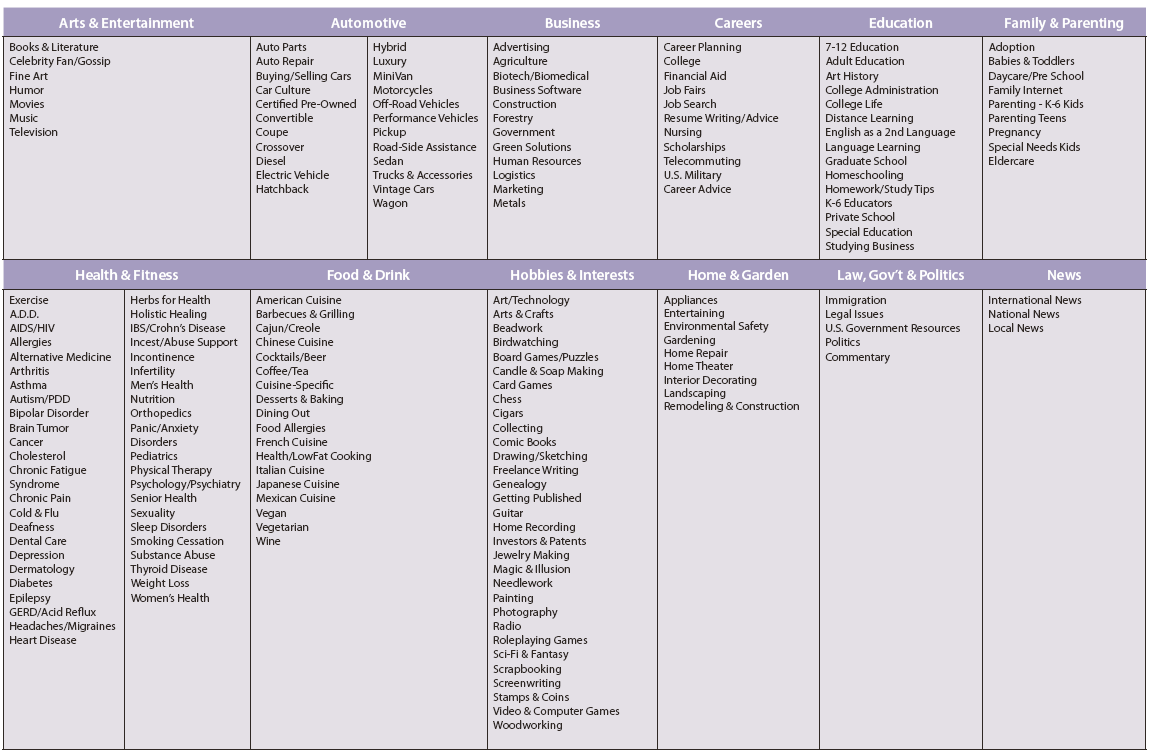
\includegraphics[width=\textwidth]{Chapters/Background/Taxonomy-1.png}
%\caption{Categories of the IAB Taxonomy}
%\label{fig:IAB1}
%\end{figure}
\end{subfigure}
\begin{subfigure}{\textwidth}
%\begin{figure}[H]
\centering
%\newline
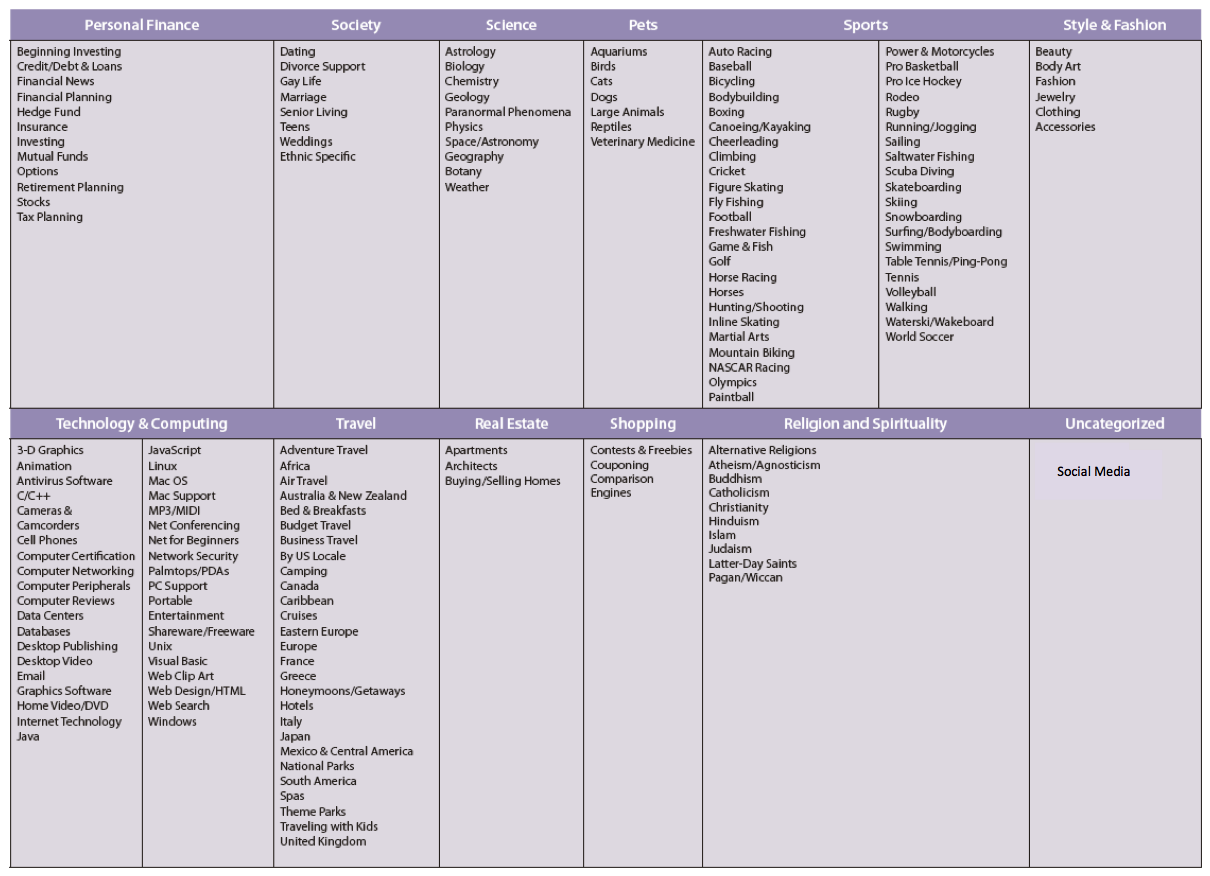
\includegraphics[width=\textwidth]{Chapters/Background/Taxonomy-2.png}
\end{subfigure}
\caption{Categories of the IAB Taxonomy}
\label{fig:IAB}
%\label{fig:IAB-categories}
\end{figure}
%Figure \ref{fig:IAB-categories} 


%When categorizing a collection of texts, similar texts will be in the same cluster and therefore in the same category. This can be used to determine the content of the text. 

%The content analysis need a list of keyword to look for in texts. 



%
\subsection{Advantages with Automatic Content Analysis}
The main advantage with automatic content analysis is time, computers work ve

\subsection{Issues}
% Main issues: 
% predefined set
% predefined keyword list
% Common knowledge -> how to represent this
Even though there are many advantages of using automatic content analysis, there are also some issues with categorization that need to be dealt with for optimal results. 
%There are some issues with automatic content analysis that are important to handle. 
The first is that the computer can only think what its learnt to think, hence cannot define its own categories but needs a predefined set of possible categories. It is a lot easier to ask the computer "Is the article about a computer scientist" than to let the computer find this possibility itself. The other issue is to decide what words are important and useful for deciding the categories of a text. 

%The computer content analysis is an automatic categorization process, where we want to find words that help us define the categories of the text. 
The first issue can be solved by defining a set of categories that we want to categorize text into. This set of categories should be presented as the desired output and be so simple that it can be understood by the users of the program. The category set should also contain a special category \textit{unknown} for texts where no category is found.
%There are some requirements that need to be met for our set; the set has to be so large that all relevant texts can be placed under at least one category, and it has to be so general that similar texts have a high probability of being categorized together. The category set should also contain a special category \textit{unknown} for texts where no category is found. 
%Another requirement for the category set is that the it has to be so well-defined and specific that it conserves as much information as possible about the categorized text. The solution to the problem should also be able to change the pre-defined category set to another pre-defined set depending on the texts that are being categorized and the context of the classification.
%that a text is not categorized under conflicting categories, for instance the category "sport" and the category "not sport". We also want the categories to be specific to have more information about the categorized text. 
%Hence the best result of the classifier would be found if the set satisfies all of these requirements with the best possible trade off between specialization and generalization. 

Feature selection is an important part of classification, and is defined as the process of selecting relevant features which will be used for the classification. It is natural to use words or phrases as features in classification of text, hence feature selection is the issue of deciding the words or phrases that are useful for categorization. These should be collected in a predefined list of keywords where our task is to create a mapping from the keywords to one or more categories that are describing for the text. The category mapping is a way of saying that a text is more likely to belong to the keyword's category if the word is present in the text. If an article mentions "Pippi Langstrømpe" (the main character in many of Astrid Lindgren's children books), the probability for the article to be about Astrid Lindgren or belong to the category "Swedish children's writers" should be larger than if the articles does not mention the name. The keyword "Pippi Langstrømpe" should therefore have some mapping to this category. 


%Input noe om wikipedia og mediawiki

\input{Chapters/Background/Challenges}

\begin{comment}
About content analysis
 - What is content analysis?
    * Automatic content analysis
 - Advantages with Automatic Content Analysis
 - Issues
    * Difficulties
 - Domain of Content Analysis 
 
Categorization 
 - What is categorization: manual vs automatic
 - Unsupervised categorization, clustering, rule-based (heuristic)
 
 Wikipedia 
  - What is Wikipedia?
 
 
 IAB 

\end{comment}
\chapter{Previous Work}
Categorization is not a new topic, neither is taking advantage of Wikipedia in the categorization process. There are many papers within the topic, hence some research have been done to avid problems already solved by others. Some of the projects have also been useful when studying their approaches for solving similar problems. This section gives a short overview of projects similar to this oe and how they solved them.

%Some of the projects have also given useful help in the task of deciding on approaches 

\section{Classification of tweets}
One of the similar projects is described in the article \emph{Entity Extraction, Linking, Classification, and Tagging for Social Media: A Wikipedia-Based Approach}\cite{entityextraction}. The initial problem described is a content analysis problem, where the goal is to categorize tweets based on their content. The chosen solution to the problem was automatic lssification of tweets, where the categorization is based on the content. This problem resemble our problem since both problems are based on understanding texts by recognizing keywords that provide information of the most likely categories. 


%where they wanted to let the computer understand what the tweets are about and then sort them based on their content. The chosen solution to the problem was to use automatic classification of the tweets, where the tweets were categorized by their content. This problem is very similar to our problem because both the problems are based on understanding texts by recognizing keywords that provide information of categories, i.e., what the tweets are about.

The article describes the categorization as the machine learning process where tweets with similar content are placed in the same class. Understanding the content requires the machine to have some basic knowledge, which is usually called a knowledge base or a repository for information. The atuhors chose to use Wikipedia as the knowledge base, for a numereous of reason, including that it is the largest online encyclopedia, that it is based on volunteering hence rapidly updated and since it is constantly crawling and therefore is able to have a fresh, dynamic and timely knowledge base. 


%The authors chose to use Wikipedia as their knowledge base (a repository for information) for finding information of the different categories. The reasons given for why they chose Wikipedia are similar to our reasons;  it is the largest online encyclopedia, it is based on volunteering which means that it is rapidly updated, and it is constantly crawling which is important since it is an advantage to have a fresh, dynamic and timely knowledge base. 

A difference between classifying tweets and articles are the preprocessing phase. Tweets require lots of preprocessing since they are quite short (max 160 characters). 


%while articles need preprocessing in order to 

The processing of the tweets required a lot of preprocessing before they could be classified content, especially since tweets are quite sort (max 160 characters).  The preprocessing of the tweets contained several steps before the actual categorization could start, including language detection, cleaning of the tweets (removing everything that is not text), and a tokenizing process (separating sentences into tokens, where a token is defined as a sequence of characters, usually normal words). The described preprocessing is similar to the preprocessing intended for our content analysis because the classifier will only find the keywords if they are an exact match. The classifier depend on tokenizing and cleaning of the words in the text to make them similar to keywords in the keyword list.  

The described tweet classification required some structure to keep information of the tweets and their possible categories. The solution was to create a structure of mentions where a mention is defined on the form ($m_{i}$, $n_{i}$, $s_{i}$), where $m_{i}$ is the string in the tweet we refer to, $n_{i}$ is the node in the knowledge base, and  $s_{i}$ is the< score of the node. All tokens with a connection to the knowledge base (i.e., Wikipedia) were considered relevant, while the others were removed to reduce the complexity. The structure of mentions could be too complex for our case with collections of texts since each text can be much longer than 160 characters, but the idea of keeping track of possible categories is the same. 

A scoring function was used for deciding categories for the tweets, where all the mentions were filtered and some hand-crafted rules were applied. Our project would also need some function to decide what categories are relevant if many categories are proposed. 



\subsection{Evaluation of the classification of tweets}
Evaluation is one of the most important part of a categorization process because it tells if the classification behaves as desired. Classification is, as already mentioned, difficult to evaluate and it was therefore quite useful to look at the evaluation part of the classification of tweets.

The authors argued that the computer classification should be compared by classification done by humans, so that the \textit{predicted} result could be compared with the \textit{correct} result. The problem is that it is very time consuming for humans to classify, so the evaluation was done by sampling 500 tweets. Of these tweets were 477 manually identified by people to give them tags which were compared by the classifier's tags. 

Figure \ref{fig:classification_entities} shows the results of the evaluation phase of the classification. The measures for each tag are P (precision: fraction of retrieved tweets that are relevant), R (recall: fraction of relevant tweets that were tagged) and F1 (F1-score: measure of accuracy, given as $ F_1 = 2 \cdot \frac{\mathrm{precision} \cdot \mathrm{recall}}{\mathrm{precision} + \mathrm{recall}}$). It is interesting to look at the results from the evaluation because they give a good indication on which subjects are difficult to classify. The results show that people and locations are easy to classify, while music is more difficult. This could be because music might contain common words that are dropped from the knowledge base or does not provide useful information while name of locations are easy to recognize for the classifier. 
%One of the most important steps of classifying is the evaluation phase. Evaluation of classifying should be done by humans. Someone will have to look through the results and see how well the classification has been done by comparing the \textit{correct} result with the \textit{predicted} result.

%The article concludes that the tweets that were easiest to classify were about people (see Figure \ref{fig:classification_entities}). This is probably because famous people have their own Wikipedia page, which is easy to match the tweet. The most difficult, on the other hand, was products which seldom have their own page  if the tweet is very specific. 


\begin{figure}[H]
\centering
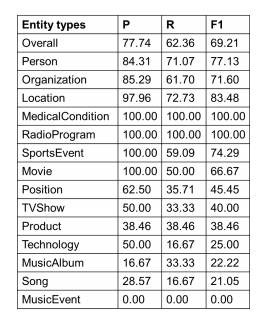
\includegraphics[height=8cm]{Classification_entities}
\caption{The accuracy of the system for extraction and linking.}
%P is the precision, R is the recall and $F_{1}$ is the $F_{1}$-score.} %linking\footnote{\url{http://pages.cs.wisc.edu/~anhai/papers/doctagger-vldb13.pdf, page 8}}}
\label{fig:classification_entities}
\end{figure}

\section{Text Categorization with Encyclopedic Knowledge}
The task of automatic content analysis has many challenges that need to be solved. 

One of the most difficult challenges is how to deal with ambiguous words or phrases. Ambiguous words are words that have more than one meaning, and the meaning is usually found from the other words in the sentence. The problem is that complex sentences and advanced grammer makes it harder for the computer to decide the meaning of a word, hence it also makes it difficult to deide the meaning of the sentence. 
%The task of making the computer understand the content of text has many difficult challenges that most humans won't encounter. Ambiguous words are for example usually not a problem for humans because it is usually easy to use the context to understand the meaning of the word. 
%Computers on the other hand depend on a dictionary or statics about the word to decide the meaning of the word. Complex sentences could also be a problem for computers, advanced grammar for example can make it difficult to interpret the meaning of the sentence.
The paper \emph{Overcoming Brittleness Bottleneck using Wikipedia: Enhancing Text Categorization with Encyclopedic Knowledge} \cite{brittleness} focus on some of these challenges and presents a solution to these. 

Some of these findings are relevant for our project or interesting for further works, hence some solutions to the common ones are mentioned here. 

One of the main problems in  content analysis performed by a computer is to decide the meaning of a word. Humans have a larger background of knowledge and experience which makes it easier to interpret the meaning of a word. Computers depend on either representing documents as bag of words (BOW) or by learning the context of the word by observation. Context is difficult for a computer because it has to decide the number of words that are needed to decide the context of a word, which obviously depends on the word. 

%Ambiguous words are foten understood from the context, but a computer is then either depending on observing the word in a similar context 

%Ambiguous words or sentences are therefore seldom a  problem for humans because the meaning can be found in the context, but a computer could encounter problems with deciding the meaning if the context is unobserved.

The paper presents a text categorization feature to make it easier for the computer to understand the meaning of a word without analysing the context. A feature is a measure for a property of the observation, for instance is number of occurrences a normal feature for each word in the  BOW. If more than one feature measured for an observation are  usually put together as a feature vector for the observation. The feature generator described in the paper takes text fragments as input and maps these to the most relevant Wikipedia articles. The concepts in the relevant articles are used to find new features, which are added to the augmented bag of words. The authors have chosen the feature generator to be a multi-resolution to generate the best relevant Wikipedia concepts, i.e., it generates features at different levels: individual word level, sentence level, paragraph level and for the whole document. This means that there is a large number of features for each document, and these features are useful to understand the content of the document. 

The feature generator depends on  a text classifier that match documents with the most relevant articles of Wikipedia. The classifier starts by manipulating the text into the same form as the encyclopedic articles. This part resembles our categorization problem since we are also interested in linking texts to Wikipedia or information from Wikipedia.  The discussion about ambiguity is also relevant for our problem, where ambiguous words should either be dropped from the keyword list or the computer will have to find the meaning of the words. 


\section{Decoding Wikipedia Categories for Knowledge Acquistion}

We have seen that the catgories contain lots of information about their pages.

This is relevant when we want to map all our Wikipedia cateogires to the desired categories . 

The paper describes ways of finding out about the content of pages based on the name of the cateogires. We could do similar in our project by using some of the same approaches. The \emph{IN} is a useful way to find all categoires .. 


\chapter{Methods}
This chapter can be viewed as an introduction to the methods we chose for the implementation of the project. It gives a brief introduction to how we determined the meaning of Wikipedia articles and the structure chosen for representing the information.

%This chapters describes methods chosen for the project and the structures 

%What do I need methods for?

\section{Finding the meaning of Wikipedia Articles}
It is essential to know the meaning of the Wikipedia articles to be able to categorize them. 
Our assumption is that the meaning of Wikipedia articles can be found by looking at the categories leading to the article in the underlying category structure of Wikipedia. We base this assumption on the fact that all Wikipedia articles are placed under at least one category, and that the articles' categories should be representative for the article. This means that we need to find a representation for the underlying structure and a way of deciding the best way of reaching each article within this structure.
%One of the most common ways
%One way of finding the meaning of WIkipedia articles is by looking at Wikipedia's underlying structure since all Wikipedia articles are placed in categories. 

% One of the most commonly used strategies of finding the meaning of the articles is by looking at the 

\subsection{Representing the underlying structure}
Taking advantage of the underlying structure of Wikipedia requires a way of representing it. Each category has links to its subcategories, and links to the articles which are placed under the category (see figure \ref{fig:graphstructure}). Representing the structure could be split into two parts; one structure representing the underlying category structure (see figure \ref{fig:categorystructure}), and one structure representing the categories of each article (see figure \ref{fig:articlestructure}).  %representing the structure between categories, and representing the structure between categories and articles. 

\begin{figure}
\centering
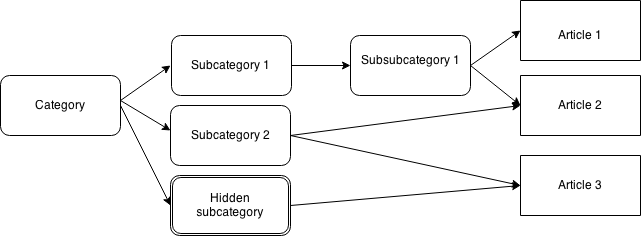
\includegraphics[width=\textwidth]{Chapters/Methods/graphstructure}
\caption{Simplified illustration of the underlying strcutre of Wikipedia.}
\label{fig:graphstructure}
\end{figure}

\subsubsection{Category graph}
A category graph is a way of representing the links between categories. This structure contains information about which subcategories can be reached from each category. Figure \ref{fig:categorystructure}) illustrates the category graph for representing the structure. The nodes in the graph (rectangles with rounded corners) represent categories, and the edges (arrows) represent the relationships between categories. The graph illustrated is a directed graph since each edge represents the relationship between the two categories (e.g. \emph{Subcategory 1} is subcategory of \emph{Category} since the arrow points from \emph{Category} to \emph{Subcategory 1}).

\begin{comment}


The graph has to contain directed edges, which means that a category is considered the subcategory of another if the category is 

can be created by representing categories as nodes and links as a 


Graph: nodes are categories and the edges are hyperlinks. 
--> nodes are categories and the edges are links between categories 


Such a graph is represented with all subcategories of a category listed under the category. The results of this is a structure like the illustration in figure \ref{fig:categorystructure}).
\end{comment}

%A category graph is a way of representing links between categories i.e., which categories can be reached from each category. The file containing all links between categories can be used to create such a graph. This is done by finding all subcategories of each category and remove all duplicate links. The results of this is a structure like the illustration in figure \ref{fig:categorystructure}).
\begin{figure}[h]
\centering
\begin{subfigure}[b]{0.4\textwidth}
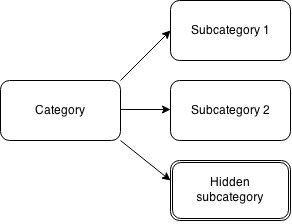
\includegraphics[width=\textwidth]{Chapters/Implementation/category-subcategories}
\caption{The structure where each category knows its subcategories}
\label{fig:categorystructure}
\end{subfigure}
\begin{subfigure}[b]{0.4\textwidth}
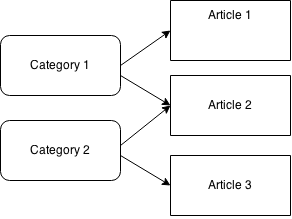
\includegraphics[width=\textwidth]{Chapters/Implementation/categories-articles}
\caption{The structure where each category know the title of its articles}
\label{fig:articlestructure}
\end{subfigure}
\caption[The representation of the Wikipedia structure]{Combined this is the structure needed to represent the Wikipedia's underlying category structure as a graph}
\end{figure}


\subsubsection{Article graph}
A different structure is desirable for representing articles and their most describing categories (the categories shown at the bottom of the article page in Wikipedia). The file containing all links between categories and their articles can be used to create a structure where each category knows its articles. Figure \ref{fig:articlestructure}) illustrates this structure. 

%It is desirable to remove articles whose titles are not relevant for our project. Numbers without context is an example of Wikipedia article titles that are difficult to determine the meaning since a number could have various meanings, including temperatures, grades or years. Hence, all article titles which only contains numbers could be disregarded. Wikipedia contains many such articles, and a total of 23 227 articles where found. This reduces the number of links betweeen articles and categories as shown in table  \ref{tab:withoutnumber}.

\begin{comment}
It is important that the category names are equal all places they occur. Wikipedia is written by volunteers from all over the worlds, and users might use different encoding depending on where they are from. Thus, both a cleaning process and a normalization process should be performed on all category names. The cleaning process is to make the category names look readable, while the normalization is a process where all words are made equal regardless of character encoding \cite[p.~26]{iirbook}.

The cleaning process includes converting all words to lowercase, replacing underscores with spaces and splitting up all titles containing the code for newline (\emph{\textbackslash n}). Newline is a way of representing how the articles should be sorted, figure \ref{fig:withnewline} is an example of an \texttt{INSERT} statement with newline in the title of the category, where the category should be sorted as if the title was \emph{ducks} as seen in figure \ref{fig:fictionalbirds}. Hence, the relevant part of the category title is the part after the newline, and this is the part that is considered further in the results. 


\begin{equation}\label{eq:removehiddencat}
a = 0
\end{equation}
\end{comment}

\subsubsection{Representing category and article names}
\emph{Id mapping} is a storage efficient way of representing category names and article titles because category names and article titles usually are longer than their representing ids. The id mapper is implemented by creating a counter that assigns a unique number to each category name or article title not already observed. 

\begin{comment}
The files containing the results becomes extremely large due to the size of the results. When writing all the results to file, the files becomes extremely large. All paths of all Wikipedia articles is more than 20 GB of compressed data. It is desirable to reduce the space needed for storing all results on the computer. The solution was to create an id mapping for each category name and article name. Id mapping gives all names a unique id, and instead of writing the full path of category names to the file, the full paths with category ids is written to file. 

The id mapping is implemented by creating a counter that assigns numbers to each category name or article name that is not found yet, i.e., a unique number represents each name. Figure \ref{fig:idmapping} shows an excerpt of the id mapping created for our purpose, where the id \emph{4600570} corresponds to the article about \emph{Ole-Johan Dahl}, which means that this id is used everywhere \emph{Ole-Johan Dahl} is used in paths. 

Id mapping is storage efficient because category names and article names usually are a  lot longer than their representing ids. 

Working with ids is also faster in many implementations concerning lookups in the program. This depends on the structure chosen for the programs, but when using dictionaries as done in our implementation, ids will perform faster than if using full names. An example of this can be seen in figure \ref{fig:id_lookup} where the time to find all categories from the category with id 177678 (corresponding to the category \emph{people}) is 0.955 minutes. Figure \ref{fig:fullname_lookup} shows the time needed to find the same paths for the category when using full names for categories and articles, which is found to be 1.559 minutes. Comparing the times shows that the time is a lot faster when using ids, which is important when many paths have to found.

The last reason to use ids instead of full names is that the full names may include characters useful for describing paths, for instance the characters "/" which is a common way of describing full paths. 

% Fordel 2: Kan bruke "/" in the text. 


\end{comment}

\section{Grading Categories}

% TODO: Find a good reference for this. 
Many Wikipedia articles can be reached from categories that are not describing for the content of the article. We found multiple paths to all Wikipedia articles, but some of them were less descriptive of the content than others. Thus, a grading was done to find the most relevant paths for each article. 

\subsection{Grading based on Inlinks and Outlinks}
%\subsubsection{Inlinks and Outlinks of Categories}
Each category in Wikipedia has a set of parent categories i.e., categories that lead to the current category, and a set of subcategories i.e., categories that can be reached from the current category. The size of these sets for a given category can be annotated as 
\begin{itemize}
\item \emph{Inlink number} = number of parent categories
\item \emph{Outlink number} = number of subcategories
\end{itemize}
Figure \ref{fig:Categorywparentandsub2} is a demonstration of how  inlink and outlink are connected to a category, and gives the idea that a catgory with high \emph{inlink} and \emph{outlink} are more likely to be visited when looking for paths for an article. 

\begin{figure}[h]
\centering

\includegraphics[width=\textwidth]{Chapters/Methods/category_parent_sub}
\caption[Example of \emph{inlink number} and \emph{outlink number} for a category]{Example of how a category has links from parent categories and links to its subcategories. The \emph{inlink number} for the category is 4 and the \emph{outlink number} for the category is 3.}
\label{fig:Categorywparentandsub2}
\end{figure}

Two assumptions can be made from this. The first assumption is that categories with high inlink number can be reached from categories that are not about the same topic. The other assumption is that categories with a high outlink number are more likely to reach articles not necessarily connected to the category name since they can reach far in all the subcategories' directions. Thus, categories with a high value of outlink and a high value of inlink should have a lower score than categories seldom reached. They cover a general topic, while categories with a low inlink number and low outlink number describe a narrow topic.

\subsubsection{Scoring paths}
Grading based on inlinks and outlinks is done by finding the number of inlinks and outlinks for all categories in the structure, and the average number of inlinks and outlinks for all categories. Then the scoring should be weighted based on the values of inlink and outlink which leads to the following equation where $\xoverline{C_{in}}$ is the average \emph{inlink} and $\xoverline{C_{out}}$ is the average \emph{outlink}.  

%The assumption that categories with high \emph{inlink} and \emph{outlink} are more often visited leads to the thought that these categories should have a lower score than categories that are more rarly visited. 

%The first approach was therefore to find the \emph{inlink} and \emph{outlink} of all categories in the structure. These numbers had to be compared with the average number of \emph{inlink} and \emph{outlink} to know whether the number is high or low (see Table \ref{tab:avginlinkoutlink}). 


\begin{equation} \label{eq:categoryscore}
Score_{C} = \frac{inlink_{c} + outlink_{c}}{\xoverline{C_{in}} + \xoverline{C_{out}}}
\end{equation}

This means that the path score of a path $P$ is the sum of the scores of all categories (see equation \ref{eq:scoreinput}). 

\begin{equation} \label{eq:scoreinput}
Pathscore_{P} = \sum_{c} Score_{C}
\end{equation}

The problem with using equation \ref{eq:scoreinput} is that short paths will be favored since there are fewer scores to be added together. A way of avoiding favoritism of short paths is by normalizing the path scores. 

\subsection{Normalized Grading based on Inlink and Outlink Numbers}
Grading based on inlink number and outlink number favors short paths even if the paths contains categories considered as bad. One way of handling this problem is by normalizing the score of each path. Equation \ref{eq:normscoreinput} is a way of normalizing the path score of path $P$ so the length of the path does not determine the relevance of the path. 

% TODO: Write something about normalization - why is it good for grading?

\begin{equation} \label{eq:normscoreinput}
Pathscore_{P} = \frac{1}{N} \sum_{c} Score_{C}
\end{equation}
where $N$ is the number of categories in the path.


\subsection{Deciding Relevant Paths}
One way of deciding which graded paths are relevant are by choosing a threshold for the path score. If the score is lower than a given threshold, it is marked as relevant, while a  higher score means that it is not relevant. A threshold can be found by deciding how many paths should be considered relevant.

One way of doing this is by finding the scores of all paths. and sort the scores from lowest to highest (see \ref{eq:sortedscores}). Then a $k$ has to be decided to how many paths are believed to be relevant of all paths, for instance one could assume that only 10\% of the paths are relevant, which leads to $k = .10 \cdot n$. 

\begin{equation} \label{eq:sortedscores}
Sorted\_scores = \left[ S_{1}, S_{2}, ... , S_{k}, ... , S_{n} \right]
\end{equation}



\begin{equation} \label{eq:threshold}
T = Sorted\_scores[k]
\end{equation}


The problem with this method is that not all articles are guaranteed to have any relevant paths. The other problem is that the score of the path will vary a lot within different fields, since some of the Wikipedia articles are categorized under very specified categories. 
% TODO: Finn en kilde som er enig med meg. 

% Problem: 
% Finne hvor mange pather som er tilgjengelig. 

Another approach is to choose the best $k$ paths for each Wikipedia article. This approach is independent of the values on other articles' path score which means all Wikipedia articles are guaranteed at least one path. The disadvantage is that some paths might be marked as relevant even though their path score is lower than path scores marked as irrelevant by other articles. Another disadvantage is that articles with many good paths will still have to choose the best $k$ paths and good paths might be lost. 

\begin{comment}
Fordeler: ser ikke på de andre
alle articler får minst en score. 

Ulemper: mange gode - hvilken er best?
Kan ikke vite om scoren er god

\end{comment}

\section{Evaluation}
An evaluation of the categorization process is essential to know whether the classifier classify correctly or not. This can also be used to find which categories are easy to classify, and which categories are difficult to recognize. The evaluation is based on comparing the results with the correct results (called \emph{Gold Standard} \cite{wiki:goldstandard}). The gold standard in our project is found in the url of articles, and is decided by the journalists when they publish articles. An article about sport contains \emph{sports} in the url, for example \emph{http://www.rappler.com/sports/by-sport/boxing-mma/pacquiao/90563-mayweather-sr-blasts-ariza}.

\subsection{Evaluation of the Classifier}
There are different ways of measuring correctness, but the most common are \emph{accuracy}, \emph{precision}, \emph{recall} and \emph{$F_{1}$-score}. These measures depend on some terms for the evaluation (see table \ref{tab:retrievedescription}).
%Evaluation the categorization is found by evaluating how well the classifier perform, in other words the correctness of the classifier.
%the correctness of the classifier
%The purpose of evaluating the classification is to determine  the correctness of the classifier 
%i.e., how well the classifier perform. 

\subsubsection{Accuracy}
\emph{Rand Index (RI)} accuracy measures the percentage of decisions that are correctly classified by the classifier \cite[p:~330]{iirbook}. Equation \ref{eq:accuracy} \cite{wiki:accuracy} shows how this is computed for evaluating the classifier. 

\begin{equation} \label{eq:accuracy}
\text{acc}=\frac{\text{true positives}+\text{true negatives}}{\text{true positives}+\text{false positives} + \text{false negatives} + \text{true negatives}}
\end{equation}

\begin{table}[ht]
\centering
\renewcommand{\arraystretch}{1.25}
\begin{tabularx}{\textwidth}{l |X}
\textbf{Term}  & \textbf{Description} \\\hline
\textbf{True Postive} (TP) & Text is classified to the class by both classifier and \emph{Gold Standard}, (correct). \\ \hline
\textbf{True Negative} (TN) &  Text is neither classified to the class by the classifier, nor by \emph{Gold Standard}, (correct).  \\ \hline
\textbf{False Negative} (FN) & Text is not classified to the class by the classifier, but by \emph{Gold Standard}, (incorrect). \\ \hline
\textbf{False Positive} (FP) & Text is classified to the class by the classifier, but not by \emph{Gold Standard}, (incorrect).
\end{tabularx}
\\[10pt]
\caption[Explanation of the \emph{TP}, \emph{TN}, \emph{FN} and \emph{FP}]{Explanation of the \emph{True Positive}, \emph{True Negative}, \emph{False Negative} and \emph{False Positive} \cite[p.~330-331]{iirbook}.}
\label{tab:retrievedescription}
\end{table}

\subsubsection{Precision and Recall}
Another way of evaluating the classifier is by using \emph{precision} and \emph{recall} which measures how many elements are correctly categorized and how many of the correct elements were found. 

%of evaluation categorization is with \emph{precision} and \emph{recall} which are measures of how many elements were correctly categorized \cite{wiki:precisionrecall}. P

Precision is defined as in equation \ref{eq:precision} \cite{wiki:precisionrecall}, which measures the fraction of returned results that are relevant \cite[p.~5]{iirbook}. This means that precision can tell how many of the articles were correctly categorized. 

\begin{equation} \label{eq:precision} 
\begin{split}
\text{precision} & =\frac{|\{\text{relevant documents}\}\cap\{\text{retrieved documents}\}|}{|\{\text{retrieved documents}\}|} \\
 & = \frac{\text{TP}}{\text{TP} + \text{FP}}
 \end{split}
\end{equation}
Recall is a measure of finding how many of the relevant documents were found \cite[p.~5]{iirbook}. Equation \ref{eq:recall} \cite{wiki:precisionrecall} would provide information about how many of the correctly categorized elements were found. 

\begin{equation} \label{eq:recall} 
\begin{split}
\text{recall} & =\frac{|\{\text{relevant documents}\}\cap\{\text{retrieved documents}\}|}{|\{\text{relevant documents}\}|} \\
 & = \frac{\text{TP}}{\text{TP}+\text{FN}}
\end{split}
\end{equation}

Combining precision and recall gives a measure of the correctness of the classifier. In addition, the measures can be combined to find the $F_{1}$-measure of the classifier which is way of measuring accuracy in terms of a weighted average of the precision and recall. The $F_{1}$-score is defined as in equation \ref{eq:fscore} \cite{wiki:fscore}. 

\begin{equation} \label{eq:fscore}
F_1 = 2 \cdot \frac{\mathrm{precision} \cdot \mathrm{recall}}{\mathrm{precision} + \mathrm{recall}}.
\end{equation}

The range of the $F_{1}$-score is between $0$ and $1$, where 1 is the best value. 

% TODO: vi kan også evaluaere mappingen mellom wikipedia articler og iab kategorier. 

%\subsection{Evaluate Wikipedia Categorization}
%\subsection{Evaluate Article Categorization}

\begin{comment}
Evaluation is the 


Kan også finne: 
p. 330 i iirbook. 
Rand index : measures the RI percentage of decisions that are correct. 
\end{comment}
\subsection{Optimize the Classifier}
%The measures for evaluating the classifier are best if they are combined. 

The measures for evaluation are used to determine how well a classifier performs and to determine how the classifier could be optimized to perform better. A perfect classifier categorizes all documents to their most describing classes without classifying documents to classes they don't belong to. Figure \ref{fig:perfect_classifier} illustrates a perfect classifier which classify all documents to their correct classes. The classification results can be seen in table \ref{tab:results_perfect_classifier}.


%This is a difficult task, and we want the classifier to achieve high scores in the evaluation.
\begin{comment}
\begin{figure}[h]
\centering
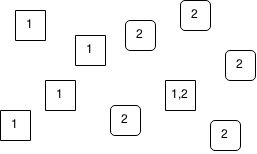
\includegraphics[width=.7\textwidth]{Chapters/Methods/All_classes}
\caption{Caption}
\label{fig:my_label}
\end{figure}

\begin{table}[h]
\centering
\renewcommand{\arraystretch}{1.25}
\begin{tabular}{c|l}
\multicolumn{2}{c}{\textbf{Number of elements in the class}} \\ \hline
\textbf{Class 1} & 5 \\ \hline
\textbf{Class 2} & 6
\end{tabular}
\\[10pt]
\caption{Caption}
\label{tab:my_label}
\end{table}

\end{comment}

\begin{figure}[h]
\centering
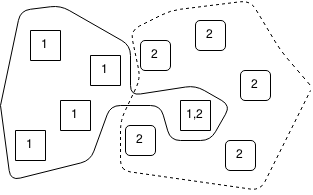
\includegraphics[width=0.7\textwidth]{Chapters/Methods/Perfect_classifier}
\caption{Illustration of a perfect classifier.}
\label{fig:perfect_classifier}
\end{figure}

\begin{table}[h]
\centering
\renewcommand{\arraystretch}{1.25}
\begin{tabular}{c|l|l|l}
\multicolumn{4}{c}{\textbf{Perfect classifier: results}} \\ \hline
\textbf{TP} & 5 &\textbf{Precision} & 1 \\ \hline
\textbf{TN} & 5 &\textbf{Recall} & 1 \\ \hline
\textbf{FP} & 0 &\textbf{Accuracy} & 1 \\ \hline
\textbf{FN} & 0 &\textbf{$F_{1}$-score} & 1
\end{tabular}
\caption{Classification results for class 1 for a perfect classifier.}
\label{tab:results_perfect_classifier}
\end{table}

\subsubsection{Why we need more than one measure for evaluation}
Creating a perfect classifier is difficult, and it is difficult to determine if the classifier perform well. The different measurements for evaluation are best when they are combined (as $F_{1}$-score), because accuracy, precision and recall can be have good results separately even if the classifier is far from perfect.  

Figure \ref{fig:high_precision}) and \ref{fig:high_recall}) illustrates classifiers that have respectively high precision and high recall. Their results can be found in table \ref{tab:results_bad_classifiers} where we can see that high precision can be found by classifier that only retrieved a few results and high recall is found for classifiers that retrieve many results. Thus, a good classifier should be neither of these, but instead balance the results. 


\begin{figure}[h]
\centering
\begin{subfigure}[b]{0.6\textwidth}
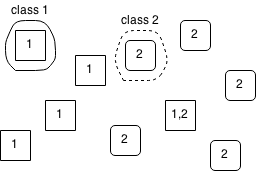
\includegraphics[width=\textwidth]{Chapters/Methods/High_precision}
\caption[Illustration of bad classifier with high precision]{Classifier A: Illustration of bad classifier with high precision.}
\label{fig:high_precision}
\end{subfigure}
\\[10pt]
\begin{subfigure}[b]{0.7\textwidth}
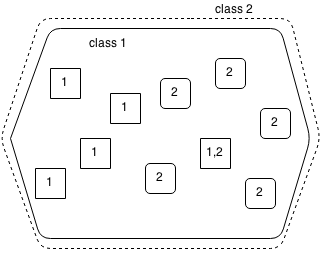
\includegraphics[width=\textwidth]{Chapters/Methods/High_recall}
\caption[Illustration of bad classifier with high recall]{Classifier B: Illustration of classifier with high recall.}
\label{fig:high_recall}
\end{subfigure}
\end{figure}


\begin{table}[h]
\centering
\renewcommand{\arraystretch}{1.25}
%\begin{tabular}{c|l|l|l|l}
%\multicolumn{2}{c}{\textbf{Classifier A}} & Classifier B \\ \hline
\begin{tabular}{l|l|l|l|l|l|l|l}
\multicolumn{4}{l}{{\bf Classifier 1}} & \multicolumn{4}{l}{{\bf Classifier2}} \\ \hline
\textbf{TP}     & 1     & \textbf{Precision}     &  1   & \textbf{TP}     & 5     & \textbf{Precision}    &   0.5  \\\hline
\textbf{TN}     & 5     & \textbf{Recall}        &  0.2   & \textbf{TN}    & 0     & \textbf{Recall}       & 1    \\\hline
\textbf{FN}     & 4     & \textbf{Accuracy}      &  0.6   & \textbf{FN}     & 5     & \textbf{Accuracy}     & 0.667    \\\hline
\textbf{FP}     & 0     & \textbf{$F_{1}$-score}      &  0.333   & \textbf{FP}     & 0     &  \textbf{$F_{1}$-score}             &    0.667
\end{tabular}
\caption{Evaluation of classifier A and B for class 1. }
\label{tab:results_bad_classifiers}
\end{table}

\begin{comment}
\begin{table}[h]
\centering
\renewcommand{\arraystretch}{1.25}
\begin{tabular}{c|l|l}
%\multicolumn{2}{c}{\textbf{Classification results for class 1}} \\ \hline
& \textbf{Classifier A} & \textbf{Classifier B} \\ \hline
\textbf{Precision} & 1 &  \\ \hline
\textbf{Recall} & 5 \\ \hline
\textbf{Accuracy} & 0 \\ \hline
\textbf{$F_{1}$-score} & 4
\end{tabular}
\caption{Caption}
\label{tab:results_high_precision}
\end{table}
\end{comment}

\begin{comment}
It is not enough to classify all documents in a class to the correct class. A perfext alskd
A classifier which categorizes all documents in a class to 
A perfect classifier categorizes all documents to the right class. We have created a classifier which might classify documents to more than one class. 
the correct results and none of the incorrect ones. 
This is a difficult task, so we try to optimize the classifier so that it retrieves most of the correct results without starting to 

The best classifier should be a classifier that retrieves m

Example of a bad classifier: It categorizes all sports article to the class sports, but also all non-sport articles to the class sport. The 

\end{comment}


\section{Wikipedia Structure}
There are two ways of accessing Wikipedia's encyclopedic information. The first way is to look up runtime as most users do when they are looking for information. The other way is more common when the information is used by other programs and

%s, which means that the program access Wikipedia's 

The other, and most common way is to download database dumps from Wikipedia. All Wikipedia articles, images and categories are stored in a database which are accessed when a user are searching for an article online. A database dump is therefore a backup of the database which are usually stored in the case of some data is lost. \footnote{TODO: reference: en.wikipedia.ort/wiki/Database\_dump} This backup is available for anyone interested at \emph{TODO: insert link}\footnote{TODO: insert reference?}. 




A database dump is defined as the table structures which is used to get the information to load

For our purpose there are some dumps that are relevant: 


I have chosen to work on the English Wikipedia, which is the largest database in with *** articles and *** pages. 

The relevant files are: 
\begin{itemize}
\item \enwikicatlink
\item \enwikipage
\item \enwikicategory
\end{itemize}

All of these files are compressed sql-files, which means that they represent files to put information into a SQL-database. Each of the files can be used to build up a database table with insert-statements, so all the information is stored in the table. 

\enwikicatlink describes all the links between categories, which describes two different types of relationships in Wikipedia. The first relationship is between a Wikipedia article and a category, i.e the category *** points to the article. The other relationship is between two categories which means that one of the categories is a subcategory of the other category. 

The file contains the table "categorylinks". Since the file is quite large (1.5GB compressed), it is desirable to split the file into two files; files containing information of the relationships between categories and files that contain information about the relationship between categories and pages. 

\section{Parsing through the dumps}
This was solved by creation the program. The program takes the \enwikicatlink as input, and goes through each INSERT-statement in the file. Since all INSERT statements contains information about many relationships, the statements are split to represent one relationship at the time. Then the statement is sorted into "Link between two categories" or "Link between a category and a page" depending on the output of the relationship described in the statement. 

Some of the information about the relationships between categories are not relevant for this problem, for instance information about hidden categories like "Unprinthworthy categories". This categories are removed in the process to reduce the number of category elements considered in the later programs. 

Wikipedia also contains lots of information about redirecting between categories and pages, for instance are article names in plural redirected to the article name in singular.  This information is also stored in \enwikicatlink and is sorted out during the process to be considered later in the process where it is desirable to redirect in the same way, but still not relevant in the early steps of the programming. 

%Category graph builder
One of the output files of the \catlinkprogram is a file containing all relationships between categories. The next step is to sort this information so that a category knows all its subcategories. The program \catgraphbuilderprogram takes the category information as output and creates a structure to represent the information. The output of the program is a file where all parents to a subcategory is stored. %This program should maybe consider loops as well
The program sorts all the categories and output a file where all subcategories of a category is listed under the name of their parent category.

\enwikicatlink also contains some shortcuts for saving space when information about the categories are inserted into the database. An example of such a statement is \footnote{TODO: insert reference: part of the insertion statement from the file \enwikicatlink}: 

\begin{code}
1517681,'fictional_birds','ducks\nfictional ducks','2014-10-26 03:30:11',
'ducks','uppercase','subcat' 
\end{code}

This part of the insertion statements means that the category \emph{fictional ducks} is both a subcategory of the category \emph{Fictional birds} and the category \emph{ducks}. This means that this statement has to result in the following information: 
\begin{code}
Fictional birds: 
* fictional ducks

ducks:
* fictional ducks
\end{code}

One of the problem in the results of the program is that there are potential for loops within the structure. This is because a category may be subcategory of a category, but also the parent category of the same category's parent. This means that the whole structure cannot be represented as a three, but is rather a graph where the connected categories are linked together. 

The other output file of \catlinkprogram is a file where the each line represents an article its immediately closest categories, these categories are the same as those represented at the bottom of the article page. 

It is desirable to get each article's full path for our problem. The next program made is therefore a program that takes creates an output where all articles and their immediate closest categories are stored. Here is also some cleaning done so that all categories which contains the words \emph{Wikipedia} or \emph{category} are removed since these are part of the hidden structure for sorting and not relevant for our task. 

To create the full path of each article are there 

the category graph and all the articles with it's 


%Article builder
After all category links are split into list describing relationships between categories and relationships between articles and their subcategories 

\subsubsection{Hidden categories}
Wikipedia's category structure contains lots of hidden categories which are not displayed at the bottom of an article page for the general users, even if the article is placed under the category. These categories are useful for editing since it is an easy way to all mark categories with something in common, for instance mark all categories with references that needs to be checked. 

Hidden categories are concerned with maintenance and administration, hence not relevant for normal users or for our problem. The next step is therefore to remove all the links to hidden categories, which led to the task of finding all hidden categories. On Wikipedia's information page about \emph{Hidden Categories}\cite{wiki:hiddencat} are 15 385 subcategories listed as immidiate subcategories, but many of these categories have links to their own hidden subcategories which also have to be found. The first attempt was to look through all the links from the category \emph{Hidden Categories}, where 15 006 subcategories where found and marked as not relevant. Since this did not give the expected number, another attempt was made by looking at the file \texttt{enwiki-latest-page\_props.sql.gz}, where figure \ref{fig:pageprops} shows how  hidden categories are marked in the table. The next attempt was therefore to find all the ids marked with \emph{hiddencat} and find the corresponding category titles in \texttt{enwiki-latest-page.sql.gz}. This approach led to 15 513 categories. To make sure that all hidden categories where found, a test was made to see if all categories from the first attempt was found in the list created from the second attempt. The results showed that all categories found in the first attempt was also found in the second attempt, and the list of all 15 513 category titles whose links should be disregarded from further results. 

\begin{figure}[h]
\centering
\begin{lstlisting}
(747593,'hiddencat','',NULL)
\end{lstlisting}
\caption[Insert statement for hidden category]{Excerpt from the file \texttt{enwiki-latest-page\_props.sql.gz} where we can see that hidden categories are marked with \emph{hiddencat}}
\label{fig:pageprops}
\end{figure}

The hidden categories have to be removed carefully because they might be subcategories of visible categories or have visible categorise as their own subcategories. An example of this can be seen in figure \ref{fig:stevie_wonder_hidden}, where the double rounded rectangle is a hidden category, the rounded rectangle is a normal (visible) category and the rectangle is the article about \emph{Stevie Wonder}.
%Hidden categories can not be disregard
%19103360 article links, 391482 category links skipped

%An example of such a structure can be found from the categories leading to the article about the singer Stevie Wonder. 

\begin{figure}[h]
\centering

\includegraphics[width=\textwidth]{Chapters/Implementation/HiddenCategories/Stevie_wonder_hidden}
\caption[Example path with hidden category]{An excerpt of one path leading to the article about to Stevie Wonder, where the path contains a hidden category. }
\label{fig:stevie_wonder_hidden}
\end{figure}

The desirable visible paths for all articles are paths without hidden categories. The next step is therefore to change the structure so that hidden categories are removed from the structure, but without loosing any of the subcategories which might contain relevant information or  important links. Example of a how a path can be transformed is figure \ref{fig:stevie_wonder} which is the excerpt from the path in figure \ref{fig:stevie_wonder_hidden} without the hidden categories. 

\begin{figure}[h]
\centering

\includegraphics[width=.7\textwidth]{Chapters/Implementation/HiddenCategories/Stevie_wonder}
\caption[Example path without hidden category]{The desirable output of the excerpt of the path leading to the article about Stevie Wonder where the hidden category is removed from the path}
\label{fig:stevie_wonder}
\end{figure}


Table \ref{tab:withouthiddencat} shows how number of links between categories, and between categories and articles are reduced when hidden categories are not considered. 

%The main reason to reduce number of links is to reduce the complexity 

\begin{table}[h]
\centering
\begin{tabular}{l|c|c}
\textbf{Links between...} & \textbf{W/ Hidden Categories} & \textbf{W/o Hidden Categories}  \\ \hline
 \textbf{subcategories} & 1 654 758  & 1 311 275\\
 \textbf{articles and categories} & 4 241 881  & 3 152 873
\end{tabular}
\caption[Number of links without hidden categories]{Number of links removed when all hidden categories are excluded. }
\label{tab:withouthiddencat}
\end{table}

\chapter{Results and Discussion}
This chapters is dedicated to evaluation of the project's results. We start by evaluating the categorization of the keywords where we tried two approaches; mapping between Wikipedia categories and output categories, and mapping between path excerpts and output categories. Further, we evaluate the performance of the dictionary-based classifier, including a section about how to retrieve the classifier's results, the different versions of the classifier, and the results from the classifier. Finally, we evaluate the Norwegian dictionary-based classifier to see how well a translated classifier perform. 


\section{Evaluation of Category Mapping}
We implemented two different approaches for mapping the Wikipedia article titles to the IAB taxonomy. The first approach was to create a mapping between Wikipedia categories and a describing category in the IAB taxonomy based on matching of words. The other approach was to create a mapping between excerpts of full paths and their most describing IAB category.

\subsubsection{Mapping from Wikipedia Categories to Output Categories}
Creating a mapping between Wikipedia categories and the IAB taxonomy was found to be difficult. The mapping was based on the matching words in the Wikipedia category with words in the IAB taxonomy, and only equal words were considered a match. A perfect result for such an approach is only achievable if the computer is able to understand natural language, i.e., know all synonyms, inflections and the true meaning of all words. There exists many projects for natural language processing, the most common is probably WordNet \cite{wordnet}, which shows that this task is a lot larger than the scope of our project. 

The other encountered with the mapping was ambiguous words in the category names. Figure \ref{fig:ambiguous_category_name} shows two categories that both contain the word \emph{Cicero}, but where the first category is for the suburb of Illinois \cite{wiki:ciceroillinois} and the other is for the Roman philosopher \cite{wiki:ciceroroman}. Creating mapping rules for these names would be a difficult or even impossible task. 

\begin{figure}[h]
\centering
\begin{lstlisting}
Category:Cicero, Illinois
Category:Cicero
\end{lstlisting}
\caption[Similar category names with different meaning]{Example of two category names which contains the same word with different meaning, and should be classified to different categories.}
\label{fig:ambiguous_category_name}
\end{figure}


The conclusion for this approach is that it might be possible to create a mapping from a Wikipedia category to one or more desirable output categories, but this would need a very specified third tier in the IAB category and lots of rules. The task would therefore resemble a manual classification and is not a desirable approach. 
%-> It is impossible to create a third tier to satisfy this. 

\subsection{Mapping from Path Excerpts to Output Categories}
Mapping between excerpts of Wikipedia category paths and IAB categories has the advantage that we can avoid ambiguity even though the category name is ambiguous. This approach is based on mapping rules between path excerpts and IAB categories. Manually creating these mapping rules  is still a tedious process. Thus, it is desirable to make the process as automatic as possible, which led to an automatic approach.

\subsubsection{Automatic mapping from path excerpts to output categories}
We started out by manually creating mappings between path excerpts and IAB categories, but this is a large task since there exists so many categories and category links in Wikipedia's structure. Thus, we tried to find a good way to predict matches between the excerpts and the output categories. We assumed that the IAB subcategory name (i.e., \emph{Auto parts}) is a category, and wanted to find the most likely categories leading to this category. This was done by finding all categories leading to this category among the top 3 category paths for each Wikipedia title, and counting the occurrences. The top 10 categories for each IAB subcategory was printed, and we kept all categories which occurred often. 

An evaluation was needed to see if the automated categorization process was successful. We decided to evaluate the automatic results for the subcategories of \emph{Automotive} with a manual classification for the same categories. Figure \ref{fig:manualclassification} is the results of the manual categorization of \emph{Automotive}, while figure \ref{fig:autoclassification1}, figure \ref{fig:autoclassification2} and figure \ref{fig:autoclassification3} represents the top 10 results automatically found for each of \emph{Automotive}'s subcategories.

%these results had to be compared to a manual categorization. We tested the automated categorization process on the category \emph{Automotive}. 

\begin{figure}[h]
\centering
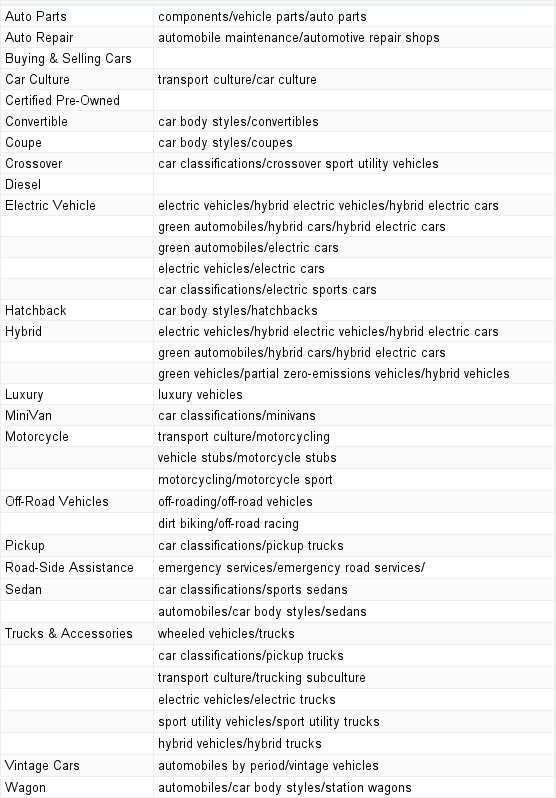
\includegraphics[width=\textwidth]{Chapters/Results/Manual_classification}
\caption[Manually mapping between categories and path excerpts]{Manually finding path excerpts for the mapping process to subcategories of \emph{Automotive}.}
\label{fig:manualclassification}
\end{figure}

\begin{figure}
\centering
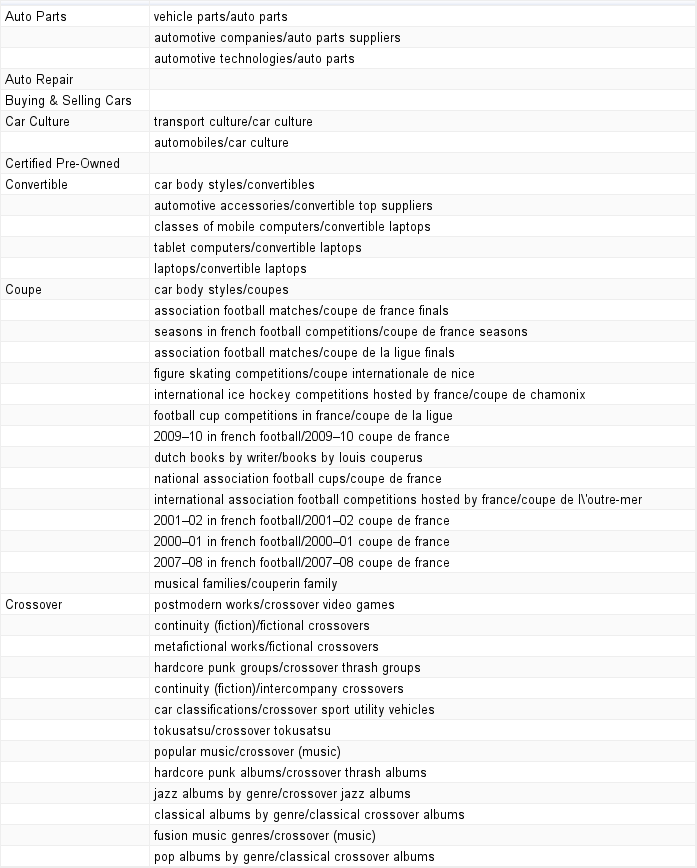
\includegraphics[width=\textwidth]{Chapters/Results/Automatic_classification_1}
\caption[Automatic mapping between categories and path excerpts, part 1]{Automatically finding path excerpts for the mapping process to subcategories of \emph{Automotive} (part 1).}
\label{fig:autoclassification1}
\end{figure}


\begin{figure}[h]
\centering
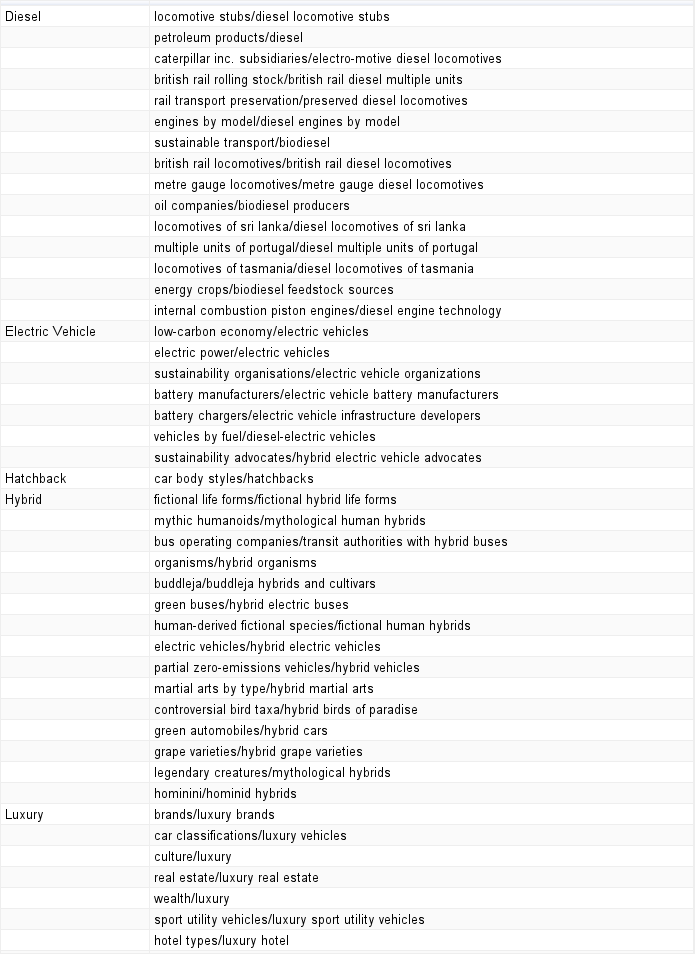
\includegraphics[width=\textwidth]{Chapters/Results/Automatic_classification_2}
\caption[Automatic mapping between categories and path excerpts, part 2]{Automatically finding path excerpts for the mapping process to subcategories of \emph{Automotive} (part 2).}
\label{fig:autoclassification2}
\end{figure}



\begin{figure}[h]
\centering
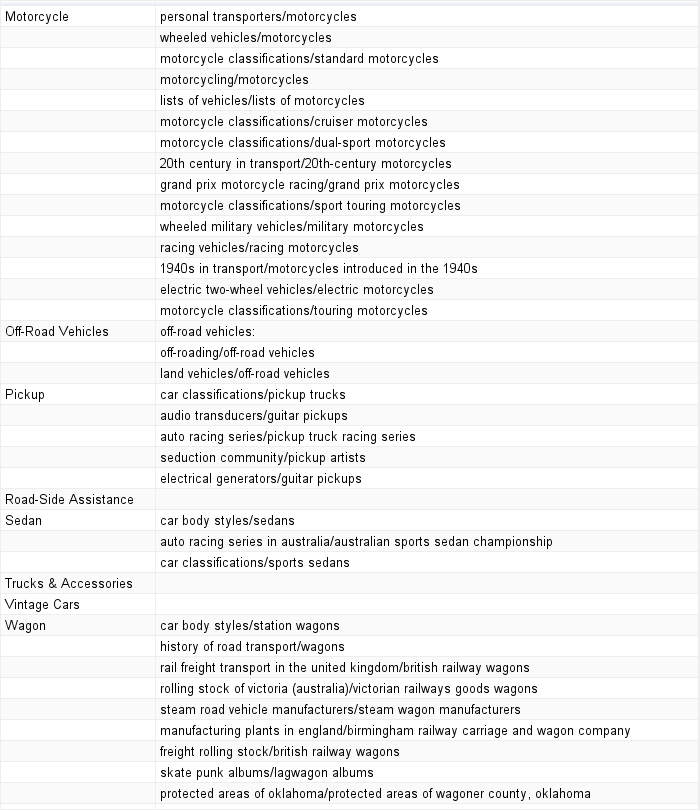
\includegraphics[width=\textwidth]{Chapters/Results/Automatic_classification_3}
\caption[Automatic mapping between categories and path excerpts, part 3]{Automatically finding path excerpts for the mapping process to subcategories of \emph{Automotive} (part 3).}
\label{fig:autoclassification3}
\end{figure}

Figure \ref{fig:wrong_automatic} illustrates a path excerpts that is not correct, which most humans will understand by common knowledge, while the computer needs lots of additional knowledge for being able to understand the same. Thus, some heuristics and human validation were needed to improve the results of the automatic categorization. 

\begin{figure}[h]
\centering
\begin{lstlisting}
Coupe:
2001-02 in french football/2001-02 coupe de france
\end{lstlisting}
\caption{Example of automatic categorization that does not work.}
\label{fig:wrong_automatic}
\end{figure}

After applying human validation, the results for \emph{Automotive} were fond in figure \ref{fig:finalclassification1} and figure \ref{fig:finalclassification2}. These results can be viewed as giving common knowledge  to the classifier, so that it is able to find patterns within the paths for categorization. Figure \ref{fig:number_of_path_excerpts_automotive} shows number of paths found for each of subcategories of Automotive, where we can see that the final results contains a higher number of path excerpts than the manual mapping, but a lower number than the automatic approach where some of the paths were removed since they were not considered relevant when validated manually.

\begin{figure}[h]
\centering
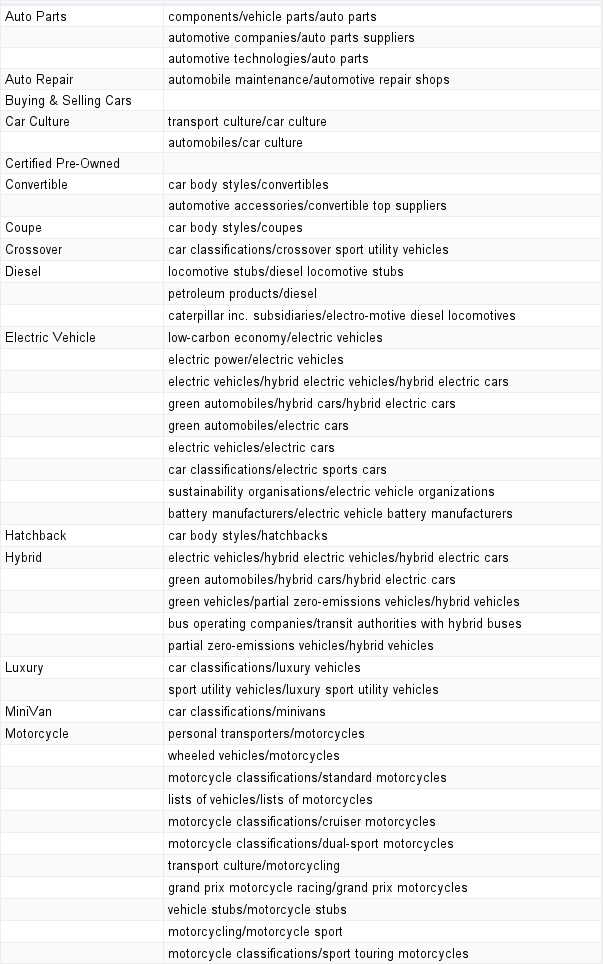
\includegraphics[width=\textwidth]{Chapters/Results/Final_classification_1}
\caption[Final results of mapping between path excerpts and IAB, part 1]{Final results of the path excerpts leading to each of \emph{Automotive}'s subcategories (part 1).}
\label{fig:finalclassification1}
\end{figure}


\begin{figure}[h]
\centering
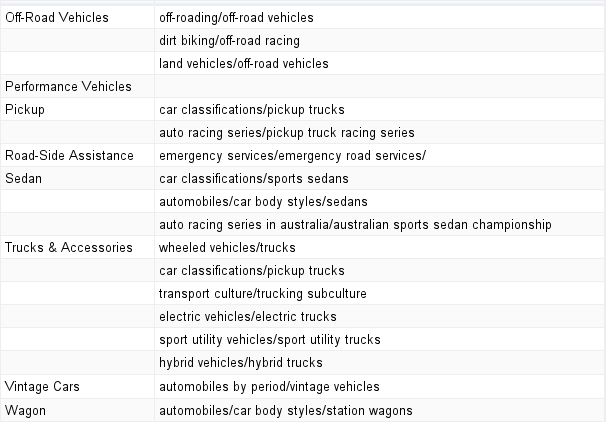
\includegraphics[width=\textwidth]{Chapters/Results/Final_classification_2}
\caption[Final results of mapping between path excerpts and IAB, part 2]{Final results of the path excerpts leading to each of \emph{Automotive}'s subcategories (part 2).}
\label{fig:finalclassification2}
\end{figure}

\begin{figure}[h]
\centering
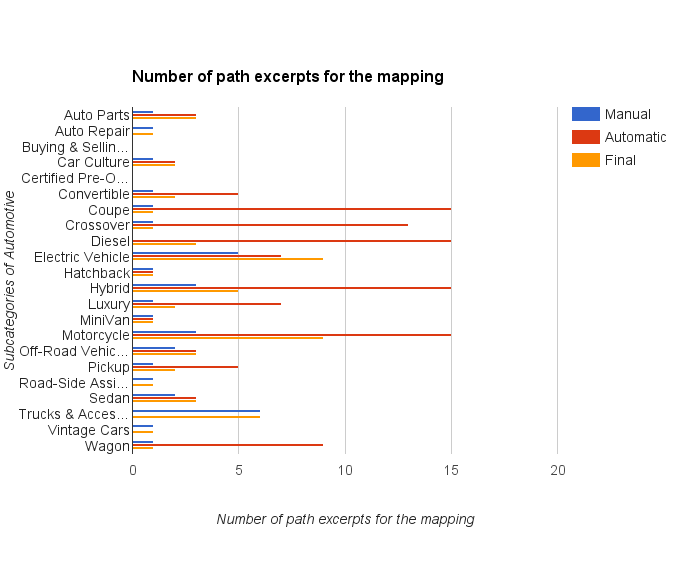
\includegraphics[width=\textwidth]{Chapters/Results/Number_of_path_excerpts_automotive}
\caption{Number of paths found for each of subcategories of Automotive. }
\label{fig:number_of_path_excerpts_automotive}
\end{figure}

\begin{comment}

Our conclusion was that it was still necessary to 

Our mapping process between path excerpts of Wikipedia categories and IAB categories has to be controlled by humans. It is desirable to make this task as automatic as possible. 

The mapping process is not completely automated since the mapping between path excerpts of Wikipedia categories and IAB categories has to be evaluated by humans. 



INSERT EXAMPLE ABOUT WALKING HERE. 
%\end{comment}

There are two main problems with manual mapping between excerpts from article paths and categories. The first problem is that the process is difficult and takes lots of time

One of the main reasons for making it an automatic process is that the process easily can be created into a 


Manually mapping between excerpts of article paths and categories is a tedious process. It is desirable to make this  process automatic or close to automatic. The reason for this is so that it is easy to create 



-automobiles/car body styles/station wagons


Eksempel på hvor variert de ulike pathene kan bli
coltainville:
* 8.72045433333 geography/geography stubs/europe geography stubs/france geography stubs/centre (region) geography stubs/eure-et-loir geography stubs/
* 8.81607333333 sports/physical exercise/dance/choreography/narratology/genres/non-fiction/non-fiction literature/historical documents/political charters/constitutions/forms of government/republics/france/geography of france/france geography stubs/centre (region) geography stubs/eure-et-loir geography stubs/
* 8.82085425    culture/cultural spheres of influence/romance countries and territories/france/geography of france/france geography stubs/centre (region) geography stubs/eure-et-loir geography stubs/


Alle:
[INFO] Total number of articles found: 152 664/4690240
[INFO] books & literature: 189169 articles



Kun 6 kategorier etter: 33 104/4690240
[INFO] books & literature: 51919 articles

-> len(cats_at_end) > 5: 

Kun 4 kategorier etter: 



\end{comment}
%\section{Evaluation}
The main purpose of the evaluation is to see whether there are any improvements when the results are applied. It is difficult to evaluate improvements, the evaluation is based on the assumption that improvement might be achieved if the categorization results are correct. 

%so evaluation of the results are performed instead. 

% Assumption: The results are good if they are correct. 

Which mapping were easy? Which where difficult and why?

- 

\begin{code}

Her må jeg skrive noe om hvordan jeg deployer resultatene til Cxense. 

\end{code}

\begin{table}[ht]
\centering
\renewcommand{\arraystretch}{1.25}
\begin{tabularx}{\textwidth}{l |c|c}
 & \textbf{sport} (iabtaxonomy) & \textbf{not sport} (iabtaxonomy)\\ \hline
 \textbf{sport} (taxonomy) & 1058 & 919 \\ \hline
 \textbf{not sport} (taxonomy) & 10516 & 99895
\end{tabularx}
\\[10pt]
\caption{}
\label{tab:}
\end{table}


\begin{comment}
Date: 15/04/15

Med: igg-iabtaxonomy-sports
     taxonomy-sports
{
  "start": 1428671088, 
  "stop": 1429103088, 
  "data": {
    "events": 185237, 
    "urls": 1058
  }
}


Med: taxonomy-sports
Uten: igg-iabtaxonomy-sports
{
  "start": 1428673680, 
  "stop": 1429105680, 
  "data": {
    "events": 105114, 
    "urls": 919
  }
}

Med: igg-iabtaxonomy-sports
Uten: taxonomy-sports
{
  "start": 1428673711, 
  "stop": 1429105711, 
  "data": {
    "events": 1875914, 
    "urls": 10516
  }
}

Uten: igg-iabtaxonomy-sports
      taxonomy-sports
{
  "start": 1428673813, 
  "stop": 1429105813, 
  "data": {
    "events": 876519, 
    "urls": 9995
  }
}

\end{comment}




It is natural to assume that there are improvements if the 

The most natural thing would be to assume that 


applying the categorization, but it is also interesting to evaluate the result of the classifier i.e., see whether it correctly assigns categories. Improvements can also be assumed to be better if the classifier has a high probability of categorize correctly.

%Evaluation of the improvement is an evaluation of the results of the user. 
%The evaluation should both cover evaluation t
%This evaluation can be thought of as two evaluation approaches; evaluation of the technical result and evaluation of the overall improvements when applying the classifier. Technical evaluation is 

%There are different parts of the result that can be evaluated,  but the most important evaluation is to evaluate the classifier to see whether it correctly assign categories. 

The evaluation of the classifier can be separated into different evaluations that together cover the whole categorization. 
%plit into different parts to get an evaluation of the different components of the classifier. 
The first evaluation could be of the predefined base components of the classifier; the keyword list and the set of categories. One way of evaluating the list of keywords is to determine if the keywords are relevant for the categorization. This could be done by looking at the size of the list i.e., how many words are included in the list, and what keywords are actually used (which occur in the collection of text). It could also be interesting to see if some of the words are never used. 

The set of categories could be evaluated as how many texts get categories to the the different categories, and try to evaluate if some of the categories seem unnecessary. The set of categories might also depend on the use of the categorization, which means that some categories might be unnecessary in some content analysis and useful in others. 

A more interesting evaluation is the function that decides what category a keyword maps to. It is not possible to do the mapping by hand since the program is operating with many thousand keywords, also in many languages, which means that the mapping has to be done automatically. The best evaluation of this function is comparing with  a true solution. Creating a true solution for the whole categorization, but there are two other approaches for evaluating the result. The first is to create a handmade solution for some small list and compare the classifier's result with this list. This will hopefully give some indication of the result of the classifier, but the result will vary a lot depending on what list we choose. 
%This should be compared by a list made by humans; what category should a keyword link to? The problem with this is that it is time consuming and difficult to make a list like this by hand. 
The other approach is to take advantage of Wikipedia's category structure. 
%
%of the list could therefore be based on Wikipedia's category structure instead. 
All articles are, as already mentioned, already categorized and it is therefore possible to compare the path 
%Since all titles are categorized is it possible to compare the path 
distances from the parent categories and to the most describing category to determine if the keyword is linking to the right categories.


The last part of the classifier's evaluation is deciding the overall result, i.e., how well does the classifier categorize the collection of texts? The best evaluation would again be to compare the classifier's result with a manual categorization and look if the results are the same. The problem with this approach is the same as with the mapping function, we need a true solution to compare with. A proposal to a result is the same; we could create a small set for comparing, but a problem with this solution is that it is a difficult task for comparing, since text can be difficult to categorize. Ole Johan Dahl could for instance be categorized under both \textit{Norwegian computer scientists} and \textit{computer scientist}, and both of them are correct. Such a comparison would therefore depend on using the same categories which can seem unnatural. It is also possible to compare the result of a classification with classifications of very similar texts to see if the categorization decides the same result. 

Some text collections can also be evaluated with help from the text itself. Lots of news articles are for instance already categorized in the URL, for instance would the URL of an article about sport contain  some information that it is about sport:\texttt{.../sport/...}. A possible solution is therefore to look the URL and see if it matches categories proposed by the classifier. 

\section{Versions of the Dictionary-Based Classifier}
It is desirable to optimize the performance of the  classifier. Thus, the classifier was improved by creating new versions of the classifier's dictionary. This section is dedicated to the different versions of the dictionary, where we focus on the improvements of each version and why these improvements were made. The variety of available categories depends on the dictionary version, because some categories are removed to focus on optimizing the results of others. %We have also described the improvements made for each version. 

\subsection{IAB Dictionary-1 (iab-1)}
The first dictionary for the classifier was an attempt to create a mapping between keywords and categories. We started by creating mapping between the categories that we thought would be easier to map from. 
\begin{comment}
\subsubsection{Available output categories}
\begin{itemize}
\item[-] automotive
\item[-] religion and spirituality
\item[-] science
\item[-] sports
\end{itemize}
\end{comment}

The results of the mapping process between keywords and categories needed to be evaluated in order to know if the mapping process worked as desired. The categories chosen at the first version were not good for evaluation with \texttt{rappler.com}. Thus, we chose to look at the 10 first keywords for each of the categories and manually classify these keywords in order to see if the results of the automatic classification was similar to the results of the manual classification. The manual classification was done by looking at the online Wikipedia article about the entry and decide the category based on the available categories from IAB. The results are shown in table \ref{tab:manual_mapping_automotive_iab-1}, \ref{tab:manual_mapping_science_iab-1}, \ref{tab:manual_mapping_religion_iab-1} and \ref{tab:manual_mapping_sports_iab-1}. The results from the manual classification shows that most of the randomly selected keywords were mapped to the same categories for both the manual and the automatic classification. Some of the keywords were also ambiguous and this was considered for the further versions. 

The main disadvantage of evaluation the manual classification is that such a small evaluation set might seem correct even though the overall results are bad. 

\begin{table}[h]
\centering
\renewcommand{\arraystretch}{1.25}
\begin{tabularx}{\textwidth}{l|X|X}
{\bf Dictionary entry}  & {\bf Automatic mapping}          & {\bf Manual mapping}                                       \\ \hline
trojan                  & automotive/vintage cars          & {\it ambiguous}                                            \\ \hline
yamaha xtz 660          & automotive/motorcycle            & automotive/motorcycle                                      \\ \hline
tatra 813               & automotive/ trucks\&accessories & automotive/ trucks\&accessories                           \\ \hline
tatra 810               & automotive/ trucks\&accessories & automotive/ trucks\&accessories                           \\ \hline
tatra 816               & automotive/ trucks\&accessories & automotive/ trucks\&accessories                           \\ \hline
tatra 815               & automotive/ trucks\&accessories & automotive/ trucks\&accessories                           \\ \hline
yamaha yz85             & automotive/motorcycle            & automotive/motorcycle                                      \\ \hline
les schwab tire centers & automotive/ {auto repair}           & automotive/auto repair \textbf{or} automotive/ trucks\&accessories \\ \hline
man truck and bus       & automotive/ trucks\&accessories & automotive/ trucks\&accessories                           \\ \hline
daryl ecklund           & automotive/motorcycle            & automotive/motorcycle \textbf{or} automotive/ crossover              
\end{tabularx}
\caption[Comparison of manual and automatic mapping, automotive]{Results for the first 10 keywords categorized to automotive with both automatic and manual mapping}
\label{tab:manual_mapping_automotive_iab-1}
\end{table}

\begin{table}[h]
\centering
\renewcommand{\arraystretch}{1.25}
\begin{tabularx}{\textwidth}{ l|X|X }
{\bf Dictionary entry}           & {\bf Automatic mapping}  & {\bf Manual mapping}                  \\ \hline
aciurina                         & science/biology          & science/biology                       \\ \hline
neurl2                           & science/chemistry        & science/chemistry                     \\ \hline
project icarus                   & science/biology          & {\it ambiguous}                       \\ \hline
darboux                          & science/space \& astronomy & science/physics                       \\ \hline
sprague                          & science/physics          & {\it ambiguous}                       \\ \hline
altenia                          & science/biology          & {\it ambiguous}                       \\ \hline
stylochyrus                      & science/biology          & {\it ambiguous}                       \\ \hline
distribution transformer monitor & science/physics          & science/physics                       \\ \hline
jarvzoo                          & science/biology          & science/biology \textbf{or} travel/theme parks \\ \hline
tomopterus similis               & science/biology          & science/biology                       
\end{tabularx}
\caption[Comparison of manual and automatic mapping, science]{Results for the first 10 keywords categorized to \emph{science} with both automatic and manual mapping}
\label{tab:manual_mapping_science_iab-1}
\end{table}


\begin{table}[h]
\centering
\renewcommand{\arraystretch}{1.25}
\begin{tabularx}{\textwidth}{ l|X|X }
{\bf Dictionary entry}   & {\bf Automatic mapping}                       & {\bf Manual Mapping}                                                                                                  \\ \hline
jean baptiste perrin     & religion\&spirituality/ atheism\&agnosticism & science/physics                                                                                                       \\ \hline
carlo mazzacurati        & religion\&spirituality/ atheism\&agnosticism & religion\&spirituality/ atheism\&agnosticism \textbf{or} arts\&entertainment/ movies                                         \\ \hline
annie laurie gaylor      & religion\&spirituality/ atheism\&agnosticism & religion\&spirituality/
atheism\&agnosticism                                                                         \\ \hline
secular ethics           & religion\&spirituality/ atheism\&agnosticism & religion\&spirituality/ atheism\&agnosticism                                                                         \\ \hline
antonio carluccio        & religion\&spirituality/ atheism\&agnosticism & food\&drinks/ italian cuisine                                                                                        \\ \hline
c. delisle burns         & religion\&spirituality/ atheism\&agnosticism & religion\&spirituality/ atheism\&agnosticism                                                                         \\ \hline
irreligion in bangladesh & religion\&spirituality/ atheism\&agnosticism & religion\&spirituality/ atheism\&agnosticism                                                                         \\ \hline
criticism of atheism     & religion\&spirituality/ atheism\&agnosticism & religion\&spirituality/ atheism\&agnosticism                                                                         \\ \hline
maryse joissains-masini  & religion\&spirituality/ atheism\&agnosticism & Law,gov't\&politics/politics                                                                                       \\ \hline
boston investigator      & religion\&spirituality/ atheism\&agnosticism & religion\&spirituality/ atheism\&agnosticism \\
& & \textbf{or} news/international news \textbf{or} \\
& &  arts\&entertainment/ books\&literature \\ 
\end{tabularx}
\caption[Comparison of manual and automatic mapping, religion]{Results for the first 10 keywords categorized to \emph{religion \& spirituality} with both automatic and manual mapping}
\label{tab:manual_mapping_religion_iab-1}
\end{table}

\begin{table}[h]
\centering
\renewcommand{\arraystretch}{1.25}
\begin{tabularx}{\textwidth}{ l|X|X }
{\bf Dictionary entry}              & {\bf Automatic mapping}  & {\bf Manual mapping}  \\ \hline
alex fong                           & sports/swimming          & {\it ambiguous}       \\ \hline
axel rauschenbach                   & sports/figure skating    & sports/figure skating \\ \hline
u.s. open - singles qualifying      & sports/tennis            & sports/tennis         \\ \hline
shooting wr sk75 junior women teams & sports/hunting\& shooting & {\it unknown}         \\ \hline
jorgen aukland                      & sports/skiing            & sports/skiing         \\ \hline
uss roebuck                         & sports/sailing           & sports/sailing        \\ \hline
davis phinney                       & sports/bicycling         & sports/bicycling      \\ \hline
ohno-group hiroshima oilers         & sports/volleyball        & sports/volleyball     \\ \hline
harry jones                         & sports/sailing           & {\it ambiguous}       \\ \hline
sunshine millions distaff           & sports/horse racing      & sports/horse racing                
\end{tabularx}
\caption[Comparison of manual and automatic mapping, sports]{Results for the first 10 keywords categorized to \emph{sports} sports by the automatic mapping, compared with the manual mapping.}
\label{tab:manual_mapping_sports_iab-1}
\end{table}

% {'science': 140740, 'religion and spirituality': 1591, 'automotive': 6664, 'sports': 87050}
\subsection{IAB Dictionary-2 (iab-2)}
We continued extending the dictionary with keyword mappings to other IAB categories because of the positive results of the simple evaluation of iab-1.  The next version of the dictionary was created with categories available for \texttt{rappler.com}, e.g., \emph{sports} and \emph{arts \& entertainment}, but we added other categories as well. 

%The results of the mapping process for iab-1 showed that the mapping process worked alright. We could argue that we only tested the results for a small sample, but it still showed that a lot of classification worked. Thus, we decided to extend the dictionary with keywords mapping to other IAB's categories, especially the categories that we could evaluate with \texttt{rappler.com} in addition to \emph{sports}, for instance \emph{arts \& entertainment}. 

\begin{comment}
\subsubsection{Available output categories}
%{'hobbies & interests': 252624, 'business': 52918, 'science': 25131, 'food & drinks': 11957, 'family & parenting': 1461, 'arts & entertainment': 266237, 'sports': 59096, 'society': 2840, 'personal finance': 3023, 'religion and spirituality': 1148, 'pets': 1530, 'automotive': 9308, 'technology & computing': 18870, 'education': 2728}
\begin{itemize}
\item[-] arts \& entertainment
\item[-] automotive
\item[-] business
\item[-] education
\item[-] family \& parenting
\item[-] food \& drinks
\item[-] hobbies \& interests
\item[-] personal finance
\item[-] pets
\item[-] religion and spirituality
\item[-] science
\item[-] society
\item[-] sports
\item[-] technology \& computing
\end{itemize}
\end{comment}

\subsection{IAB Dictionary-3 (iab-3)}
We noticed that almost all articles were mapped to the category \emph{science} in iab-2. The reason for this was that process of cleaning the dictionary entries were done after we had removed all the common words. This lead to some problems if the processed dictionary entry was a common word (example: figure \ref{fig:common_word} where \emph{(85476) 1997 MY} was reduced to \emph{my}, which is also a common English word). 

\begin{comment}
\subsubsection{Available output categories}
%{'hobbies & interests': 252624, 'business': 52918, 'science': 25131, 'food & drinks': 11957, 'family & parenting': 1461, 'arts & entertainment': 266237, 'sports': 59096, 'society': 2840, 'personal finance': 3023, 'religion and spirituality': 1148, 'pets': 1530, 'automotive': 9308, 'technology & computing': 18870, 'education': 2728}
\begin{itemize}   
\item[-] arts \& entertainment
\item[-] automotive
\item[-] business
\item[-] education
\item[-] family \& parenting
\item[-] food \& drinks
\item[-] hobbies \& interests
\item[-] personal finance
\item[-] pets
\item[-] religion and spirituality
\item[-] science
\item[-] society
\item[-] sports
\item[-] technology \& computing
\end{itemize}
\end{comment}

\subsection{IAB Dictionary-4 (iab-4)}
The results of the classifier showed that it classified few articles correctly. We looked at the results and realized that the classifier favoured short paths. Thus, we decided to normalize the grading of the paths (equation \ref{eq:normscoreinput}). The results of the classifier (see section \ref{sec:results_from_classifier}) shows that more articles were correctly categorized after the normalization were performed (from * to ** correctly categorized articles for \emph{arts \& entertainment}). 

%We noticed that too many articles were categorized to \emph{arts \& entertainment} and decided to temporarily remove this category. 
\begin{comment}
\subsubsection{Available output categories}
%{'automotive': 9146, 'food & drinks': 11650, 'family & parenting': 1442, 'arts & entertainment': 246744, 'sports': 58591, 'society': 2713, 'personal finance': 2981, 'science': 24300, 'technology & computing': 18509, 'education': 2669}
\begin{itemize}
\item[-]arts \& entertainment
\item[-]automotive
\item[-]education
\item[-]family \& parenting
\item[-]food \& drinks
\item[-]personal finance
\item[-]science
\item[-]society
\item[-]sports
\item[-]technology \& computing
\end{itemize}
\end{comment}

\subsection{IAB Dictionary-5 (iab-5)}
%We noticed that too many articles were categorized to \emph{arts \& entertainment}. Some 

\subsection{IAB Dictionary-6 (iab-6)}
The results for iab-5 showed that there were still too many articles assigned to the category \emph{arts \& entertainment}. The reason for this was that many keywords for this category are titles of movies, songs or books which contains common words. We decided to remove all entries that contained \emph{any} common words from our dictionary. This reduced the number of dictionary entries from ** to  ***.  The disadvantage of removing all entries that contain a common word is that we might loose information from our dictionary, but the advantage is that it might help with disambiguation of phrases that might be both common sentences and a dictionary entry. 

\begin{comment}
\subsubsection{Available output categories}
%{'automotive': 9039, 'food & drinks': 11512, 'family & parenting': 1429, 'arts & entertainment': 251585, 'sports': 58274, 'society': 2703, 'personal finance': 2966, 'science': 23894, 'technology & computing': 18357, 'education': 2668}
\begin{itemize}
\item[-]arts \& entertainment
\item[-]automotive
\item[-]family \& parenting
\item[-]food \& drinks
\item[-]education
\item[-]personal finance
\item[-]science
\item[-]society
\item[-]sports
\item[-]technology \& computing
\end{itemize}
\end{comment}

\begin{comment}
\subsection{IAB Dictionary-7 (iab-7)}
The results of the classification showed that we still got too many articles classified as \emph{Arts \& Entertainment}. Thus, we did some exploration to determine the reason for this. 


The results shown that many dictionary entries were common words that were classified as \emph{Arts \& Entertainment}. These words were not among the most common words, but were still too common to be used as dictionary entries. Examples of such words were 
\begin{itemize}
\item peaceful
\item tuseday
\item maps
\end{itemize}
This problem was mostly found for \emph{Arts \& Entertainment} and we decided to remove all entries that were classified to the class \emph{Arts \& Entertainment} where the entry was a single word. A total number of 38846 %18168

entries were removed from the dictionary version by this approach. 

\end{comment}

\subsection{All Dictionary Versions}
The process of creating new dictionary versions for each classifier shows that the classifier was improved for each version. Some categories were added for a dictionary version to advance the variety of the classifier, and some categories were removed in order to focus on improving other categories. Table \ref{tab:available_categories} shows the available categories for each version of the classifier. Each version had different number of entries per categories as seen in figure \ref{fig:numberofentriespercat}. It is also noticeable that we decided on fewer entries per category for the later versions of the dictionaries, where more ambiguous entries were removed.  


\begin{figure}[h]
\centering
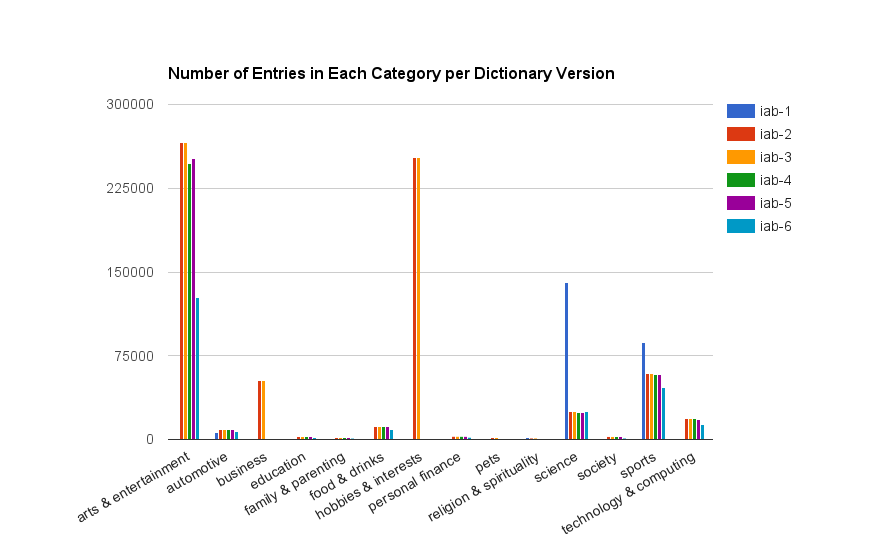
\includegraphics[width=\textwidth]{Chapters/Results/Numberofentriespercat}
\caption[Number of entries per category for each dictionary version]{Number of entries per category for each of our dictionary versions. Notice that not all categories are present in all versions.}
\label{fig:numberofentriespercat}
\end{figure}

\begin{comment}
We noticed that not all ambiguous entries were removed from the dictionary in version \emph{iab-5}. Thus, we collected all ambiguous category articles which are found under the category \emph{All ambiguous pages} (a total of *** pages). 




\end{comment}

\begin{table}[h]
\centering
\renewcommand{\arraystretch}{1.25}
\begin{tabular}{l|l|l|l|l|l|l}
                                & {\bf iab-1} & {\bf iab-2} & {\bf iab-3} & {\bf iab-4} & {\bf iab-5} & \textbf{iab-6} \\ \hline
{\bf arts \& entertainment}     &             & X           & X           & X           & X & X       \\ \hline
{\bf automotive}                & X           & X           & X           & X           & X & X       \\ \hline
{\bf business}                  &             & X           & X           &             &   &         \\ \hline
{\bf education}                 &             & X           & X           & X           &   &         \\ \hline
{\bf family \& parenting}       &             & X           & X           & X           & X & X       \\ \hline
{\bf food \& drinks}            &             & X           & X           & X           & X & X       \\ \hline
{\bf hobbies \& interests}      &             & X           & X           &             &   &         \\ \hline
{\bf personal finance}          &             & X           & X           & X           & X & X       \\ \hline
{\bf pets}                      &             & X           & X           &             &   &         \\ \hline
{\bf religion and spirituality} & X           & X           & X           &             &   &         \\ \hline
{\bf science}                   & X           & X           & X           & X           & X & X       \\ \hline
{\bf society}                   &             & X           & X           & X           & X & X       \\ \hline
{\bf sports}                    & X           & X           & X           & X           & X & X       \\ \hline
{\bf technology \& computing}   &             & X           & X           & X           & X & X       \\ 
\end{tabular}
\caption{Available categories for each dictionary version. }
\label{tab:available_categories}
\end{table}


\begin{comment}
Number of entries: 
iab-1: 693933
iab-2: 693933 ????
iab-3: 4487442
iab-4: 1141214
iab-5: 1153967
\end{comment}

% TODO: Insert something about the different versions

\section{Results from Classifier}
\label{sec:results_from_classifier}
The main purpose of the evaluation is to see whether there are any improvements when the results are applied. We assumed that improvements are found if the classifier categorized correctly. This section is dedicated to evaluating the results automatically from \texttt{rappler.com}.

%This section describes how we validate the classifier's results 

\subsubsection{Rappler.com}
Our project was tested at the webpage \texttt{www.rappler.com} which is an online Indonesian news site where most articles are written in English. Articles on Rappler are sorted by the publishers based on the articles' contents. The available categories and their subcategories are shown in table \ref{tab:rapplercontent}.

\begin{table}[ht]
\centering
\renewcommand{\arraystretch}{1.25}
\begin{tabularx}{\textwidth}{l|  X }
\textbf{Main category} & \textbf{Subcategories} \\ \hline
News & Philippines, World, \#BalikBayan, Science \& Nature, Specials \\ \hline
Video & Newscast, Shows, Reports, Documentary, Specials \\ \hline
Business & Economy, Brighter Life, Industries, Money, Features, Specials \\ \hline
MoviePH & Issues, \#ProjectAgos, \#BudgetWatch, \#HungerProject, Community, IMHO \\ \hline
Views & Thought Leaders, iSpeak, Rappler Blogs, \#AnimatED \\ \hline
Life \& Style & Food, Books, Arts \& Culture, Travel, Specials, \#PugadBaboy \\ \hline
Entertainment & Entertainment News, Movies, Music, Special Coverage \\ \hline
Sports & Boxing, Basketball, Football, Other Sports, University Sports\\ \hline
Tech & News, Features, Reviews, Hands on, Social Media \\ \hline
Live & \#RStream, Newscast \\ \hline
BrandRap & Stories, Specials, \#BuildWealth, \#HomeMagic, \#BrighterLife, \#BetterWorld
\end{tabularx}
\\[10pt]
\caption{Rappler's category structure}
\label{tab:rapplercontent}
\end{table}
We have focused on 3 categories which are present both on Rappler and in IAB's taxonomy, i.e., \emph{Sports}, \emph{Entertainment} and \emph{Tech/Technology}. These categories are evaluated for all versions of the classifier to see how well the classifier performed and to see if any improvements were made between the different versions. 

\subsubsection{Bias with our evaluation}
Some of Rappler's articles are not written in English. These articles cannot be classified by our classifier since it is based on an English dictionary. Selection of all English articles is done by only looking at articles that contain the tag "language":"en". 

% TODO: Hva med de som er publisert før vi startet klassifiseringen?
%be classified correctly by our classifier due to 


\subsection{Retrieving Results from Cxense}
Our classifier's results were retrieved from \emph{Cxense insight} by finding all articles with the tag we are looking for. We chose to only look at the results from the last 5 days \footnote{The last results retrieved for evaluation was retrieved *** of July 2015.}. Figure \ref{fig:retrievecode} shows an example of code for  retrieving all articles which contain the tag \emph{sports} within both the url taxonomy and \emph{igg-iabtaxonomy5}. 

\begin{figure}[h]
\centering
\begin{lstlisting}
{ "siteId":"9222338298879175891", 
"groups":["url"],
"start":"-5d",
"fields":["urls"],
"filters":[
{"type":"keyword","group":"'igg-iabtaxonomy5'","item":"'sports'"},
{"type":"keyword", "group":"taxonomy","item":"'sports'"}],"count":1000}'
\end{lstlisting}
\caption[Example of code for retrieving results]{Example of code for retrieving all events with \emph{sports} within the url taxonomy and within igg-iabtaxonomy5.}
\label{fig:retrievecode}
\end{figure}



\subsection{Weight for Classification}
Another issue is to decide the boundaries of the classification, i.e., minimum number of keyword occurrences necessary for categorizing an article to a class. A boundary can be found by looking at weights for the tag in articles. This means that only articles which contain a tag with at least a certain weight will be returned. The question is to determine the minimum weight for these articles. 

We tested different minimum weight values to determine when the classifier returned the best results. This was tester  for dictionary version iab-6 and the article tag \emph{sports}. The results of the test can be viewed in table \ref{tab:classification_results_weights} and \ref{tab:classification_evaluation_weights}. The results showed that the classifier performed best with a minimum weight of 0.5 or 0.6. It is possible to see the trade-off between precision and recall in table \ref{tab:classification_results_weights}

\begin{table}[h]
\centering
\renewcommand{\arraystretch}{1.25}
\begin{tabularx}{\textwidth}{l |X|X|X|X|X|X|X|X|X}
         & {\bf 0.1} & {\bf 0.2} & {\bf 0.3} & {\bf 0.4} & {\bf 0.5} & {\bf 0.6} & {\bf 0.7} & {\bf 0.8} & {\bf 0.9} \\ \hline
{\bf TP} & 305       & 159       & 159       & 159       & 159       & 122       & 122       & 69        & 69        \\ \hline
{\bf TN} & 18207     & 18952     & 18959     & 18959     & 18952     & 19066     & 19066     & 19197     & 19224     \\ \hline
{\bf FP} & 972       & 279       & 279       & 279       & 142       & 142       & 46        & 46        & 1         \\ \hline
{\bf FN} & 1445      & 1595      & 1595      & 1598      & 1598      & 1638      & 1640      & 1683      & 1743    
\end{tabularx}
\caption[Classification results for different minimum weights.]{Classification results for iab-6 and sports with different values of minimum weight.}
\label{tab:classification_results_weights}
\end{table}


\begin{table}[h]
\centering
\renewcommand{\arraystretch}{1.25}
\begin{tabularx}{\textwidth}{l |X|X|X|X|X|X|X|X|X}
               & {\bf 0.1} & {\bf 0.2} & {\bf 0.3} & {\bf 0.4} & {\bf 0.5} & {\bf 0.6} & {\bf 0.7} & {\bf 0.8} & {\bf 0.9} \\ \hline
{\bf Precison} & 0.239     & 0.363     & 0.363     & 0.363     & 0.363     & 0.462     & 0.462     & 0.600     & 0.857     \\ \hline
{\bf Recall}   & 0.174     & 0.091     & 0.091     & 0.090     & 0.090     & 0.069     & 0.069     & 0.039     & 0.003     \\ \hline
{\bf Accuracy} & 0.884     & 0.910     & 0.912     & 0.911     & 0.911     & 0.915     & 0.915     & 0.918     & 0.912     \\ \hline
{\bf F1-score} & 0.202     & 0.145     & 0.145     & 0.145     & 0.145     & 0.121     & 0.120     & 0.074     & 0.006     
\end{tabularx}
\caption[Evaluation scores for different minimum weights.]{Evaluation scores for iab-6 and sports with different values for minimum weight.}
\label{tab:classification_evaluation_weights}
\end{table}


\begin{table}[h]
\centering
\renewcommand{\arraystretch}{1.25}
\begin{tabular}{l|l|l}
\textbf{Category}               & \textbf{iab-3}    & \textbf{iab-6}    \\ \hline
\textbf{sports}                 & 1.322314          & 31.755811         \\ \hline
\textbf{arts \& entertainment}  & 7.112775          & 15.968101         \\ \hline
\textbf{technology}             & 1.473297          & 16.393443
\end{tabular}
\caption[Improvement in $F_{1}$-score in newer classifier versions]{Improvement in $F{1}$-score when comparing version 3 and version 6 of the classifier for all three evaluation categories.}
\label{tab:improved_f1}
\end{table}



\subsection{Results for Sports}
We started by evaluating the results for the IAB category \emph{sports} for the different versions of the classifier.\footnote{The 1st version of the classifier did not have any classification rules for sports.} The results are shown in \ref{tab:iabresults_sports}, while the evaluation scores are shown in \ref{tab:precision_sports}. 

\begin{table}[h]
\centering
\renewcommand{\arraystretch}{1.25}
\begin{tabularx}{\textwidth}{l|  X|X|X|X|X|X }
         & {\bf iab-1} & {\bf iab-2} & {\bf iab-3} & {\bf iab-4} & {\bf iab-5} & {\bf iab-6} \\ \hline
{\bf TP}        & NaN       & 131         & 16          & 15          & 294         & 567         \\ \hline
{\bf TN}        & NaN       & 25852       & 26613       & 26606       & 26539       & 26034       \\ \hline
{\bf FN}        & NaN       & 2269        & 2379        & 2379        & 2091        & 1839        \\ \hline
{\bf FP}        & NaN       & 719         & 9           & 8           & 80          & 598         \\ 
\end{tabularx}
\\[10pt]
\caption[Classification results for \emph{sports}]{Classification results for all versions of the classifier for the category \emph{sports}.}
\label{tab:iabresults_sports}
\end{table}

\begin{table}[h]
\centering
\renewcommand{\arraystretch}{1.25}
\begin{tabularx}{\textwidth}{l|  l|l|l|l|l|l }
                & {\bf iab-1} & {\bf iab-2} & {\bf iab-3} & {\bf iab-4} & {\bf iab-5} & {\bf iab-6} \\ \hline
{\bf Precision} & NaN         & 15.411765   & 64.000000   & 65.217391   & 78.609626   & 48.669528   \\ \hline
{\bf Recall}    & NaN         & 5.458333    & 0.668058    & 0.626566    & 12.327044   & 23.566085   \\ \hline
{\bf Accuracy}  & NaN         & 89.686238   & 91.770342   & 91.771236   & 92.514826   & 91.607549   \\ \hline
{\bf F1-score}  & NaN         & 8.061538    & 1.322314    & 1.241208    & 21.312070   & 31.755811   \\
\end{tabularx}
\\[10pt]
\caption[Categorization results for \emph{Sports}]{Evaluation scores for the different versions of the classifier when classifying \emph{sports}.}
\label{tab:precision_sports}
\end{table}


\subsubsection{Evaluation of the results}
The results of the classification show that all evaluation scores are better in the later versions of the dictionary, where \emph{iab-5} and \emph{iab-6} are the versions with best results. 

The main difference between \emph{iab-5} and \emph{iab-6} is that there are fewer entries in \emph{iab-6} than in \emph{iab-5}. It is noticeable that \emph{iab-5} has a higher number of correctly classified articles (TP), but also a higher number of wrongly classified articles (FP). Classifier \emph{iab-6}, on the other hand, has a higher recall which means that it has less wrongly classified articles. 




Comparison with other projects. 



\subsection{Results for Arts \& Entertainment}
The online web page used for evaluation (\texttt{rappler.com}) contains a category called \emph{Entertainment}, which corresponds to the IAB taxonomy's category \emph{Arts \& Entertainment}. Thus, we retrieved all classified results for evaluating how well the classifier performed when classifying entertainment related articles. The classification results are shown in table \ref{tab:iabresults_entertainment} and the evaluation scores are shown in table \ref{tab:precision_entertainment}.

\begin{table}[h]
\centering
\renewcommand{\arraystretch}{1.25}
\begin{tabularx}{\textwidth}{l|  X|X|X|X|X|X }
         & {\bf iab-1} & {\bf iab-2} & {\bf iab-3} & {\bf iab-4} & {\bf iab-5} & {\bf iab-6} \\ \hline
{\bf TP} & NaN          & NaN           & 152         & 154         & 2530        & 2543        \\ \hline
{\bf TN} & NaN          & NaN           & 25090       & 24990       & 1196        & 39          \\ \hline
{\bf FN} & NaN          & NaN           & 2398        & 2396        & 23          & 1           \\ \hline
{\bf FP} & NaN          & NaN           & 1572        & 1683        & 25489       & 26764       \\
\end{tabularx}
\\[10pt]
\caption[Classification results for \emph{arts \& entertainment}]{Classification results for all versions of the classifier for the category \emph{arts \& entertainment}.}
\label{tab:iabresults_entertainment}
\end{table}

\begin{table}[h]
\centering
\renewcommand{\arraystretch}{1.25}
\begin{tabularx}{\textwidth}{l|  X|X|X|X|X|X }
                & {\bf iab-1} & {\bf iab-2} & {\bf iab-3} & {\bf iab-4} & {\bf iab-5} & {\bf iab-6} \\ \hline
{\bf Precision} & NaN         & NaN         & 8.816705    & 8.383234    & 9.029587    & 8.677108    \\ \hline
{\bf Recall}    & NaN         & NaN         & 5.960784    & 6.039216    & 99.099099   & 99.960692   \\ \hline
{\bf Accuracy}  & NaN         & NaN         & 86.409695   & 86.041816   & 12.743690   & 8.798174    \\ \hline
{\bf F1-score}  & NaN         & NaN         & 7.112775    & 7.020743    & 16.551093   & 15.968101   \\
\end{tabularx}
\\[10pt]
\caption[Evaluation scores for \emph{arts \& entertainment}]{Evaluation scores for the different versions of the classifier when classifying \emph{arts \& entertainment}.}
\label{tab:precision_entertainment}
\end{table}

\subsubsection{Evaluating the results}



\subsection{Results for Tech}

\begin{table}[h]
\centering
\renewcommand{\arraystretch}{1.25}
\begin{tabularx}{\textwidth}{l|  X|X|X|X|X|X }
         & {\bf iab-1} & {\bf iab-2} & {\bf iab-3} & {\bf iab-4} & {\bf iab-5} & {\bf iab-6} \\ \hline
{\bf TP} & NaN              & NaN           & 4           & 4           & 24          & 70          \\ \hline
{\bf TN} & NaN              & NaN           & 28692       & 28683       & 28664       & 28458       \\ \hline
{\bf FN} & NaN              & NaN           & 530         & 529         & 509         & 465         \\ \hline
{\bf FP} & NaN              & NaN           & 5           & 3           & 51          & 249         \\
\end{tabularx}
\\[10pt]
\caption[Classification results for \emph{technology}]{Classification results for all versions of the classifier for the category \emph{technology}.}
\label{tab:iabresults_technology}
\end{table}

\begin{table}[h]
\centering
\renewcommand{\arraystretch}{1.25}
\begin{tabularx}{\textwidth}{l|  X|X|X|X|X|X }
                & {\bf iab-1} & {\bf iab-2} & {\bf iab-3} & {\bf iab-4} & {\bf iab-5} & {\bf iab-6} \\ \hline
{\bf Precision} & NaN         & NaN         & 44.444444   & 57.142857   & 32.000000   & 21.943574   \\ \hline
{\bf Recall}    & NaN         & NaN         & 0.749064    & 0.750469    & 4.502814    & 13.084112   \\ \hline
{\bf Accuracy}  & NaN         & NaN         & 98.169751   & 98.179267   & 98.085339   & 97.558307   \\ \hline
{\bf F1-score}  & NaN         & NaN         & 1.473297    & 1.481481    & 7.894737    & 16.393443   \\
\end{tabularx}
\\[10pt]
\caption[Evaluation scores for \emph{technology}]{Evaluation scores for the different versions of the classifier when classifying \emph{technology}.}
\label{tab:precision_technology}
\end{table}


\subsubsection{Evaluating the results}
\section{Discussion of the Results}
The results of our classifier shows that all versions of the classifier categorizes too many articles to all classes, i.e., too many false positive (FP) for each class. The main reason for this is that we have created a one-to-many classifier, i.e., our dictionary-based classifier can assign more than one class to each article, while we compare with a one-to-one classification, i.e., each article is placed under one class in its url structure. This means that articles might be evaluated as wrongly classified even though the results of the classifier is correct. 

\begin{comment}


There are many reasons why the results are 


- dårlig 
- flere klassser
- tvetydige ord. 


are 2 main reasons for this: 
\begin{enumerate}
\item Many articles concern more than one topic: An article about a musician playing golf would be most likely be categorized as both entertainment and sports by our classifier, while the journalist publishing the article would have to choose the category within the url structure.  
\item The required number of keywords for assigning a class is too low: We could all occurrences of keywords within the class, and it might be more realistic to put a lower limit before the category is assigned to the article. 
\end{enumerate}


\end{comment}
\section{Evaluation of the Norwegian Classifier}
We also needed to evaluate the results from the Norwegian classifier. It would be very interesting to compare the results of the "translated" dictionary with a dictionary-based classifier created by the same approach as the English classifier. This was not possible due to the projects deadline. Thus, the evaluation of the Norwegian classifier is performed by retrieving the classification results in the same way as evaluation of the English classifier. 


\begin{table}[h]
\centering
\renewcommand{\arraystretch}{1.25}
\begin{tabular}{l |l|l}
         & {\bf sports} & {\bf arts \& entertainment} \\ \hline
{\bf TP} & 165          & 687                         \\ \hline
{\bf TN} & 18030        & 14461                       \\ \hline
{\bf FP} & 1677         & 1243                        \\ \hline
{\bf FN} & 92           & 3359                        \\
\end{tabular}
\\[10pt]
\caption{Classification results for the category \emph{Sports}.}
\label{tab:results_norwegian}
\end{table}



\begin{table}[h]
\centering
\renewcommand{\arraystretch}{1.25}
\begin{tabular}{l |l|c}
                & {\bf sports} & \multicolumn{1}{l|}{{\bf arts \& entertainment}} \\ \hline
{\bf Precision} & 64.202335    & 16.979733                                        \\ \hline
{\bf Recall}    & 8.957655     & 35.595855                                        \\ \hline
{\bf Accuracy}  & 91.139050    & 76.698734                                        \\ \hline
{\bf F1-score}  & 15.721772    & 22.991968                                        \\
\end{tabular}
\\[10pt]
\caption{Classification results for the category \emph{Sports}.}
\label{tab:evaluation_norwegian}
\end{table}

\begin{comment}
\subsubsection{Results for \emph{Sports}}

\begin{table}[h]
\centering
\renewcommand{\arraystretch}{1.25}
\begin{tabular}{l|l}
 & \textbf{no-iab} \\ \hline
\textbf{TP} & 1342 \\ \hline
\textbf{TN} & 87657 \\ \hline
\textbf{FN} & 23252 \\ \hline
\textbf{FP} & 1240 
%\end{tabularx}
\end{tabular}
\\[10pt]
\caption{Classification results for the category \emph{Sports}.}
\label{tab:no_classifier_sports_results}
\end{table}

\begin{table}[h]
\centering
\renewcommand{\arraystretch}{1.25}
%\begin{tabularx}{\textwidth}{l| l }
\begin{tabular}{l|l}
                        & \textbf{no-iab}   \\ \hline
\textbf{Precision}      & 0.520             \\ \hline
\textbf{Recall}         & 0.055             \\ \hline
\textbf{Accuracy}       & 0.784             \\ \hline
\textbf{$F_{1}$-score}  & 0.099
%\end{tabularx}
\end{tabular}
\\[10pt]
\caption{Evaluation results for the IAB category \emph{Sports}.}
\label{tab:no_classifier_sports_scores}
\end{table}

\subsubsection{Results for \emph{Arts \& Entertainment}}

\begin{table}[h]
\centering
\renewcommand{\arraystretch}{1.25}
%\begin{tabularx}{\textwidth}{l|l }
\begin{tabular}{l|l}
 & \textbf{no-iab} \\ \hline
\textbf{TP} & 3972 \\ \hline
\textbf{TN} & 77778 \\ \hline
\textbf{FN} & 5586 \\ \hline
\textbf{FP} & 23806
%\end{tabularx}
\end{tabular}
\\[10pt]
\caption{Classification results for the category \emph{Arts \& Entertainment}.}
\label{tab:no_classifier_entertainment_results}
\end{table}

\begin{table}[h]
\centering
\renewcommand{\arraystretch}{1.25}
%\begin{tabularx}{\textwidth}{l| l }
\begin{tabular}{l|l}
                        & \textbf{no-iab}   \\ \hline
\textbf{Precision}      & 0.143             \\ \hline
\textbf{Recall}         & 0.416             \\ \hline
\textbf{Accuracy}       & 0.680             \\ \hline
\textbf{$F_{1}$-score}  & 0.213
%\end{tabularx}
\end{tabular}
\\[10pt]
\caption{Evaluation scores for the IAB category \emph{Arts \& Entertainment}.}
\label{tab:no_classificer_entertainemtent_scores}
\end{table}



\begin{comment}
precision = 1342/(1342+1240) = 0.51975213013
recall = 1342/(1342+23252) = 0.05456615434
accuracy = (1342 + 87657)/(1342 + 87657 + 23252 + 1240) = 0.7841943414
f1 = 2(0.51975213013*0.05456615434)/(0.51975213013+0.05456615434) = 0.09876361494



Kultur: 
TP: 3972
FN: 5586
FP: 23806
TN: 77778
precision: 3972/( 3972 + 23806) = 0.14299085607
recall: 3972/(3972 + 5586) = 0.41556811048
accuracy: (3972 + 77778)/(3972+77778 + 5586+32806) = 0.68044480697
f1: 2( 0.14299085607*0.41556811048) /(0.14299085607 + 0.41556811048) = 0.21277051638

\begin{table}[]
\centering
\begin{tabular}{c|c}
 &  \\
 & 
\end{tabular}
\caption{Caption}
\label{tab:my_label}
\end{table}
\end{comment}

\chapter{Conclusion and Further Work}
There are both improvements and desirable further work available for this study. 

%that could be added to this solution. 

\section{Conclusion}
\subsection{Summary (of essay)}
This paper has given a brief introduction to the automatic categorization problem used for content analysis. The main reason for automatic content analysis isthat manual classification is impossible for large collections of text, since it is both time consuming and  depends on experts within the topic of the texts. Automatic content analysis is based on the idea that the computer understands texts by recognizing specific keywords that  connected to one or more predefined categories. The advantages of basing such a keyword list on the titles of articles from Wikipedia is that Wikipedia is a large online encyclopedia that covers lots of subjects and is regularly maintained by lots volunteers. The category set for the classification can vary depending on the purpose of the classification, but it is essential that the predefined set is large enough to cover enough topics, but also so specific that information is preserved. An example of a predefined category set that is well-suited for advertisement is provided by IAB, Interactive Advertising Bureau. 

\subsection{The final results}
\section{Further Works}
There exists many desirable extensions for our dictionary-based classifier that might improve the results or expand the usage. The most important future improvements for our classifier is solving ambiguity in a better way and extending the dictionary by exploring more than just the titles of Wikipedia articles. Expanding the usage is possible if the classifier is well-defined for other languages than just Wikipedia. 

\subsubsection{Disambiguation}
Our project removed all ambiguous titles. This means that we loose information that might be valuable for classification purposes. Instead of removing the titles, we could keep the titles that are most relevant for our classification, for instance the titles that have the longest articles. We studied different projects for solving disambiguation, and some of their findings could be applied to find the most likely meaning of an ambiguous entry. 

\subsubsection{Stubs}
Another possible change for the program is to remove Wikipedia stubs. Wikipedia stubs are pages that are too short to be considered articles. Wikipedia contains 1 913 507 stubs \cite{wiki:allstubs}, and these articles might provide ambiguous information which are more likely to be removed since they contain so little information that they are not considered articles.  


\subsubsection{Explore more information from Wikipedia}
We have only looked at the titles when creating the dictionary-based classifier. Another extension would be to explore the actual content of the articles before they are classified to the most describing categories. Better categorization of the Wikipedia articles could lead to better results for the classifier, which could improve the results. 

\subsubsection{Adding information}
We have only used information from Wikipedia, but it might be desirable to extend our classifier with information in addition to Wikipedia. Keywords from other sources might improve the results like it did in \cite{entityextraction} when adding information from MusicBrainz, City DB, Yahoo! Stocks, Chrome and Adam. 

\subsubsection{Improve Mapping}
The mapping between keywords and categories could also be improved by creating better decision rules between category paths and IAB categories. We chose to grade our Wikipedia article titles by using inlink and outlink number. Another improvement could be to try other grading algorithms, which might be better for determining the content of the articles. 
%It could also be improved by trying other grading algorithms. 

\subsubsection{Extending for more languages}
The results and implementation is created for English Wikipedia, hence only useful for English articles. We created a Norwegian dictionary-based classifier by using the internal Wikipedia links to translate the English classifier's dictionary to Norwegian. We noticed that the Norwegian classifier lacked important information for being able to classify Norwegian articles, and concluded that this is probably because special Norwegian keywords are missing from the dictionary. 

Thus, a desirable extension would be to create a more general approach for creating the dictionary so that it could be applied to other languages as well. Most of our programs are not dependent on language, except for the mapping rules. A good extension would be to create a language independent mapping process which could create dictionary-based classifiers from Wikipedia in multiple languages. 


%\subsection{Automatic mapping from Wikipedia titles}
%The mapping process from Wikipedia and to desirable output is a 





%It has discussed the different components needed to perform a content analysis on a collection of texts. Two of the most important components of the classifier has been discussed; a predefined list of keywords where the keywords are based on the titles of Wikipeda, and a predefined set of categories for the result. The paper has also discussed important properties of the predefined category set, followed by other similar work and discussion of evaluation of the classifier, i.e., what parts of the classifier can be evaluated and how this should be done. 

\backmatter{}
\cleardoublepage
\renewcommand{\bibname}{References}
%%\bibliography{mybib}

%\cleardoublepage

\addcontentsline{toc}{chapter}{References}
\printbibheading
\printbibliography[keyword=ref,heading=subbibliography,title={Main References}]
\printbibliography[keyword=wikipedia,heading=subbibliography,title={Wikipedia References}]

%e={Wikpedia Reference%\printbibliography[title={References},keyword=ref]

%\printbibliography[title={Wikipedia References},keyword=wikipedia]

%\printbibliography[keyword=primary, title={Primary references}]
%\printbibliography[notkeyword=primary, title={Other references}]


% Fra Sigmund:
%%\bibliographystyle{plain}

% 2. Clear double page. This is necessary to produce the correct page number for the
%    Bibliography-entry in the table of contents. This will however not resolve the problem with the
%    hyperlink of this entry in the table of contents, which will still refer to the previous
%    chapter/section/subsection in the table of contents (this could be fixed by adding the
%    BibTeX-file before including the Bibliography-entry (step 3), but then the page number will be
%    incorrect again).

% 3. Add the Bibliography-entry to the table of contents.


%%\bibliography{mybib}
\end{document}
